\documentclass[12pt]{report}
\usepackage[T1]{fontenc}
\usepackage[utf8]{inputenc}
\usepackage{natbib}
\setcounter{secnumdepth}{3}
\setcounter{tocdepth}{3}
\usepackage{textcomp}
\usepackage{graphicx}
\usepackage{nomencl}
\usepackage[french]{babel}
\usepackage{hyperref}
%\usepackage[cyr]{aeguill}

\frenchbsetup{og = «, fg = »}

% the following is useful when we have the old nomencl.sty package
\providecommand{\printnomenclature}{\printglossary}
\providecommand{\makenomenclature}{\makeglossary}
\makenomenclature

\makeatletter

%%%%%%%%%%%%%%%%%%%%%%%%%%%%%% LyX specific LaTeX commands.
\DeclareFontEncoding{LGR}{}{}
\DeclareRobustCommand{\greektext}{%
  \fontencoding{LGR}\selectfont\def\encodingdefault{LGR}}
\DeclareRobustCommand{\textgreek}[1]{\leavevmode{\greektext #1}}
\ProvideTextCommand{\~}{LGR}[1]{\char126#1}

%% Special footnote code from the package 'stblftnt.sty'
%% Author: Robin Fairbairns -- Last revised Dec 13 1996
\let\SF@@footnote\footnote
\def\footnote{\ifx\protect\@typeset@protect
    \expandafter\SF@@footnote
  \else
    \expandafter\SF@gobble@opt
  \fi
}
\expandafter\def\csname SF@gobble@opt \endcsname{\@ifnextchar[%]
  \SF@gobble@twobracket
  \@gobble
}
\edef\SF@gobble@opt{\noexpand\protect
  \expandafter\noexpand\csname SF@gobble@opt \endcsname}
\def\SF@gobble@twobracket[#1]#2{}
%% A simple dot to overcome graphicx limitations
\newcommand{\lyxdot}{.}


%%%%%%%%%%%%%%%%%%%%%%%%%%%%%% Textclass specific LaTeX commands.
\newenvironment{lyxlist}[1]
{\begin{list}{}
{\settowidth{\labelwidth}{#1}
 \setlength{\leftmargin}{\labelwidth}
 \addtolength{\leftmargin}{\labelsep}
 \renewcommand{\makelabel}[1]{##1\hfil}}}
{\end{list}}

\@ifundefined{date}{}{\date{}}
\makeatother


%\makeatletter
%\addto\extrasfrench{%
%   \providecommand{\og}{\leavevmode\flqq~}%
%   \providecommand{\fg}{\ifdim\lastskip>\z@\unskip\fi~\frqq}%
%}
%
%\makeatother
\begin{document}
%\title{{*}}

%\maketitle
\begin{titlepage}
 \begin{center}
    {\Large
     Zürcher Hochschule der Künste ZHdK\\
 	en collaboration avec l'Interkantonale Hochschule für
        Heilpädagogik HfH \\
	 Upgrade MAS in Klinische Musiktherapie \\ Master of Advanced Studies en musicothérapie clinique\\}
  \vfill
  {\Huge \emph{Le potentiel du test d'écoute Tomatis\textsuperscript \textregistered  pour la 
  musicothérapie} 
  	\vfill%Essai et réflexions en musicothérapie\\ sur des sujets souffrants de troubles de l'humeur 
  %au moyen d'un test d'écoute}
} \medskip


{\LARGE The Potentiel of the Tomatis\textsuperscript \textregistered Listening Test for  Music Therapy } 
\vfill

{\Large Mémoire pour l'obtention du titre de\\ \medskip
Master of Advanced Studies in Klinische Musiktherapie \\ \smallskip 
présenté par Valérie Gaillard}

{\large Directrice de mémoire : Bettina Kandé-Staehelin}



	 \hfill \\
	 \rule{0mm}{1pt} \hfill
{\large Zürich, novembre  2020}
 \end{center}
\end{titlepage}

% !TEX root = ./master.tex

\begin{abstract}
	\centerline{\textbf{Abstract}}
	\begin{french}	
\textbf{L'axe principal} porte sur la comparaison de la faculté d'écoute des patients avant et après 
la  musicothérapie.
\textbf{Les outils:} le test d'écoute Tomatis et le questionnaire WHOQOL sur la qualité de vie sont 
utilisés 
pour synthétiser les différences  pré/post traitement.
 %Des graphiques de courbes d'écoute synthétisent des différences pré/post traitement.
 13 patients, avec difficulté de régulation des émotions, sont répartis en 2 groupes: 6 patients avec la  
 musicothérapie et  7, de contrôle.
 % Le WHOQOL est rempli avant et 
 %après séjour afin d'évaluer leur état psychique.
\textbf{Résultats:} l'analyse comparative des résultats révèle une modification positive et significative 
d'écoute pré/post traitement %par le 
%test 
%d'écoute 
%Tomatis
 pour le groupe de 
musicothérapie, confirmée par le  WHOQOL, contrairement au groupe contrôle où la transformation est
faible et le questionnaire majoritairement négatif. % avec des valeurs plus 
%élevées. 
%Pour le groupe contrôle, la transformation a été faible et le questionnaire majoritairement 
%négatif.
\textbf{Conclusions:} la musicothérapie a eu un impact positif sur la transformation de l'écoute, corrélée 
à l'état psychique mis en évidence par le WHOQOL.
\textbf{Remarque:}  la totalité des tests d'écoute et des questionnaires demeure 
inférieur à ce qui avait été initialement planifié, et, en dépit d'une plus ample dimension statistique, ce 
travail avantagera plus les aspects qualitatifs que quantitatifs. %d'être 
%statistiquement significatifs, rendant notre travail plus qualitatif que quantitatif.
%Ayant tout à fait conscience des compétences scientifiques qu'une telle étude aurait exigé, ce travail 
%oscillera 

\textbf{Mots-clés: musicothérapie; écoute; son; oreille; test}
\end{french}

\begin{english}	
\textbf {The main axis} is about the observation by comparison of the auditory perception faculty of 
patients during the outcome of music therapy.
\textbf{Tools:} Tomatis listening test and WHOQOL quality of life questionnaire.
Listening curve graphs summarize the difference before and after treatment.
13 patients with the same type of pathology (difficulty in regulating
emotions) are divided into 2 different groups: one experimental group of 6 patients following music 
therapy, and one control group of 7 patients. Patients fill out the WHOQOL questionnaire before and after 
treatmenas to determine the impact or the lack of impact of the therapy on their listening.
\textbf{Results:} analysis of observation shows a positive and significant modification for the music 
therapy group regarding the WHOQOL test. The post-therapy questionnaire indeed shows an increase in 
values compared to the pre-therapy one.
For the control group, the transformation was weak and the questionnaire was mostly negative.
\textbf{Conclusions:} Music therapy had a positive impact on the transformation of listening, correlated 
to the psychic state, as the WHOQOL questionnaires results clearly showed.
\textbf{Note:} the small study added to the final number of WHOQOL lower than expected prevent our 
results from being statistically 
significative.
% the final number of listening tests and WHOQOL test was found lower than expected. 
%Added to the fact this was a small study. This therefore prevents our results from being statistically 
%significative. 
%Being fully aware of the scientific skills that such a study would’ve required, 
This work will oscillate more 
towards the qualitative aspect of the study than the quantitative.
\textbf{Keywords: music therapy; listen; sound; hear; test}
\end{english}
\end{abstract}













%\begin{Remerciements}

\tableofcontents
%  à DéVELOPPER
\chapter{Introduction et Hypothèse : }
\begin{quotation}
\emph{Par le Son, le Silence du Non-Être vient à l'Être. Je suis
la musique que je fais ou écoute. La musique a la capacité d'harmoniser
les composantes d'une entité psychophysique pour qu'il soit ``bien
dans sa peau'' et ``bien dans son âme''}\footnote{Jacques Viret, \emph{B. A-BA de la musicothérapie}, \cite{Viret2007}.}.
\end{quotation}
J'exerce le métier de musicienne professionnelle depuis de nombreuses
années. Par la suite, je suis aussi devenue musicothérapeute, formée
également en tant que consultante à la méthode Tomatis, études suscitées
par mon intérêt croissant au sujet du développement de la personne
à travers l'outil que nous offre la musique : le son.

Dans ma pratique, les deux formations ont successivement pris plus
ou moins d'importance, selon les périodes de travail en clinique psychiatrique,
en réhabilitation à la SUVA, ou selon mon travail dans mon cabinet
privé. En clinique, ce sera exclusivement la musicothérapie. En cabinet
privé, j'aurai la liberté de choix dans l'utilisation des deux méthodes.
C'est ainsi que, peu à peu, à travers chaque cas particulier du patient,
j'ai vu mes techniques d'approche et de soin se modifier, évoluer,
pour parfois, aller se fusionner. Dans ce cheminement, de nombreuses
interrogations se sont imposées et continuent de m'interpeller.

Ce qui m'a animée? C'est de creuser et d'approfondir mes recherches.
Pourrai-je être plus précise dans mes observations? Pourrai-je
clarifier ma manière de travailler qui est celle de mixer les deux
méthodes ?

\section{Hypothèse: un test d'écoute comme outil musicothérapeutique}


En partant de l'utilisation d'un test d'écoute spécifique employé dans
la thérapie Tomatis, l'hypothèse suivante s'est imposée à moi : ce
test d'écoute pourrait-il servir aux musicothérapeutes? Y aurait-il
moyen de donner un champ de \emph{vision de l'écoute} du patient suivi
exclusivement en musicothérapie ? Pourrait-il être un outil
intéressant ?


Ce domaine est très vaste et la façon d'utiliser les sons et de les
traiter l'est aussi. L'objet de cette étude est de faire un constat
qui pourrait donner matière à réflexion tout en ne confrontant pas les
différentes techniques employées --- qui pourraient avoir plus ou % un grand tiret ---
% un tiret entre no de pages: pp. 23--40
moins d'impact quant à l'évolution du travail du patient.

Ma recherche est celle-ci : est-il pertinent d'utiliser ce test
d'écoute Tomatis en musicothérapie sans utiliser les outils propres à
cette méthode ? Il n'y aura pas d'utilisation de l'Oreille
électronique ni des musiques préparées et filtrées.  Un support
graphique, visible, presque ``palpable'', avec des critères
d'interprétations, pourrait-il donner une ``dessin'', une image utile,
utilisable, tangible ? Permettrait-il de visualiser plus objectivement
les changements, la transformation de l'écoute du patient et la
démonstration de ce travail? % quel travail?
un travail % quel travail
qui mettrait à jour une perception différente, une sensibilité
nouvelle?

Ne serait-ce % qui est 'ce' et 'là'?
pas là en définitive une forme de démonstration du
travail de la musicothérapie?  Il nous semble que ce soit une
question importante car la musicothérapie est souvent mal comprise car
en définitive mal connue par définition. % pourquoi par définition?
La crédibilité d'une thérapie
passe souvent par des preuves. Mais est-ce que la musique, invisible
et légère, qui constitue le médium utilisé en musicothérapie, laisse
des traces extérieures?
% Une psychothérapie aussi ne laisse pas de traces physiques. Mais on peut
% en mesurer les effets.
Elle est utilisée dans le but d'un processus
thérapeutique, pour entrer en communication avec soi-même dans un
premier temps, et pouvoir ensuite mieux percevoir le monde qui nous
entoure, communiquer et s'exprimer\footnote{%
Voir ce lien sur \href{http://www.musictherapy.ch/fr/musicotherapie/quest-ce-que-la-musicotherapie/}{musictherapy.ch}}.
L'aspect intemporel du son, de la musique, de ce médium volatil par
définition en comparaison avec l'art-thérapie, ne pourra apporter le
même aspect concret que peuvent témoigner des supports graphiques,
visuels, reflets d'un espace-temps lors d'un travail d'élaboration
psychique d'un patient.  Nous gageons que l'action et l'impact de la
musicothérapie pourraient être perçus, d'une certaine façon plus
clairement, saisis comme dans l'\oe il de l'objectif d'un appareil
photographique, vus et constatés, et ce, en priorité dans l'esprit du
patient pour et par lui-même.

En tant que musicothérapeute, nous ne pouvons nous servir des outils
scientifiques tel que l'IRMfct; par contre, toutes ces recherches en
neurosciences appuient et renforcent la crédibilité de l'action
majeure du son sur notre cerveau.  Emmanuel Bigand, professeur de
psychologie cognitive à l'Université de Bourgogne, relève l'aspect
paradoxal de la musique, la complexité de sa structure sonore sans
fonction biologique précise mais faisant réagir fortement l'être
humain. ( chap.3 p.35, E.Bigand," Vous avez l'oreille musicale" ,Le
cerveau mélomane, Ed.Belin) Notre cerveau peut être activé autant par
la musique que par la nourriture ou la drogue. Et pourtant la musique,
élément artificiel en soi, n'a aucun rôle dans notre survie ni dans
notre nutrition.


\section{Plan du travail}

Dans la première partie, j'aborderai l'aspect théorique : l'écoute, le test d'écoute, les différents sortes de tests d'écoute en musicothérapie, (Verdeau-Paillès, Auriol). Nous aborderons aussi brièvement l'anatomie de l'oreille. Ensuite, nous expliquerons la méthode Tomatis,
et puis, beaucoup plus en détail, son test d'écoute.

En deuxième partie ce sera l'aspect clinique : les tests faits en clinique avec deux groupes de
comparaison.

Et finalement suivront la vérification de l'hypothèse, les conclusions et interrogations.
 
\chapter{L'écoute}

\section{Ecouter ou entendre : une différence}

La définition du verbe ``entendre'' et du verbe ``écouter'', 
\footnote{dictionnaire Hachette, édition 2012 }nous paraît opportune % opportune?
en raison de la confusion courante des deux termes :
\begin{description}
\item[Entendre] c'est  percevoir des sons, saisir par l'ouïe
\item[Ecouter] a trois sens: 
\begin{enumerate}
	\item prêter l'oreille pour entendre
	\item prêter attention
	à l'avis de quelqu'un, suivre un avis
	\item \emph{fig}: suivre une impulsion,
	une inspiration.
\end{enumerate}
\end{description}



\emph{Entendre} est une attitude passive par rapport au monde sonore
qui nous entoure. Nous recevons les sons sans les interpréter et cela
ne demande aucun effort. C'est une action involontaire et non
sélective.

    Selon Bernard Auriol,\textit{entendre} \begin{quote}
	suppose un son (physique), une oreille
	pour le capter, un système nerveux pour le recevoir.
\end{quote} Tandis qu' \textit{écouter }\begin{quote}
	est un
	processus actif supposant préférences et répulsions pour tel son ou
	telle séquence sonore.
\end{quote}\footnote{\cite{Auri96:clesons}.}.

Entendre et écouter sont «deux
fonctions essentiellement distinctes bien qu'évoluant apparemment sur
des terrains identiques\footnote{Extrait de l'entretien réalisé par
	Bernard Auriol avec Alfred Tomatis, 1973.}.» ... avec «l'élément conscient, facteur essentiel sur lequel repose toute la
différence entre ces deux activités».
\begin{quote}
	``(...) Entendre n'implique pas pour autant la présence d'un champ
	conscient.\emph{ Entendre, c\textquoteright est en quelque sorte subir
		un son }ou un message qui nous est adressé. \emph{Ecouter, c'est désirer
		appréhender ce son }ou ce message . (...)'' 
	
	\footnote{Professeur Tomatis \char`\"{}Education et Dyslexie\char`\"{} Editions
		ESF Collection \char`\"{}Sciences de l'éducation\char`\"{}.}
\end{quote}


Ainsi \emph{écouter} est une opération de tout autre nature
puisqu'elle suppose une participation active dans le choix du message
ou dans la sélection d'une voix. Elle  implique la volonté,
permet une forme de décodage: il s'agit d'une capacité. Dans un milieu sonore important, bruyant, comme un café, lorsque nous lisons attentivement, nous faisons abstraction
des bruits environnants; en soi, nous les entendons parfaitement mais nous n'y
prêtons pas attention. Nous parvenons à couper les sons parasites, à nous en abstraire pour
nous concentrer que sur les plus  pertinents, en l'occurrence ici  notre lecture intérieure.
Nous savons qu' "écouter" a des origines sanskrites et signifie "partager"; nous remarquons alors à juste titre que nous écoutons le plus souvent en face de quelqu'un pour pouvoir dialoguer et échanger, et que le même phénomène se réalise avec un livre qui transmet et partage des connaissances. L'écoute permet la communication, sous-entend la présence de quelqu'un et nécessite de la  concentration. Il faut cette volonté incluse dans la concentration pour comprendre et rentrer en contact avec la voix de  l'écrivain qui chante dans le texte avec celle, intérieure,  du lecteur.

 





\emph{Ecouter} se base certes sur une stimulation prenant sa source à
l'extérieur mais \emph{devant être intérieurement, intentionnellement
  recherchée}.




\section{Le son}
\begin{quotation}
	\char`\"{}\textbf{C'est le son qui a fabriqué l'oreille et si tu veux connaître
	le son, apprends d'abord à étudier l\textquoteright oreille\char`\"{}.}
	Hermès Trimégiste
\end{quotation}

Le son possède plusieurs caractéristiques physiques. Il peut être
défini très précisément par un ensemble d'unités physiques chiffrées
: les décibels et les hertz. 
\begin{itemize}
	\item Un décibel est l'unité de mesure de l'intensité du son. Un décibel
	est égal à 1/10 de bel ; une augmentation de l'intensité égale à 1
	bel équivaut à peu près à un doublement de l'intensité sonore. 
	\item Un hertz est une unité de fréquence\footnote{la fréquence est le nombre de vibrations par unité de temps dans un
		phénomène périodique} (symbole : Hz). Équivalent à 1 s-1. Fréquence d'un phénomène périodique
	dont la période est une seconde. Ses multiples sont, entre autres,
	le kilohertz (kHz), le mégahertz (MHz) et le gigahertz (Ghz). Cette
	unité vient du savant allemand Heinrich Hertz, pionnier de la radioélectricité.
\end{itemize}
Le son peut être défini de deux manières : 
\begin{itemize}
	\item d'une manière objective tout d'abord : c'est le phénomène physique
	d'origine mécanique consistant en une variation de pression (très
	faible), de vitesse vibratoire ou de densité du fluide, qui se propage
	en modifiant progressivement l'état de chaque élément du milieu considéré,
	donnant ainsi naissance à une onde acoustique (la propagation des
	ronds dans l'eau suite à un ébranlement de la surface donne une bonne
	représentation de ce phénomène) ; 
	\item d'une manière subjective également : il s'agit de la sensation procurée
	par cette onde, qui est reçue par l'oreille, puis transmise au cerveau
	et déchiffrée par celui-ci.\index{http://www.futura-sciences.com/sante/dossiers/medecine-bruit-effets-sante-259/page/3}
\end{itemize}
De plus, il y a de nombreux paramètres en prendre en compte : par
exemple : l'impression de force sonore : la sensibilité de l'oreille
est une variable de la fréquence. Il faut 1000 fois moins de pression
acoustique pour avoir une sensation auditive à 4000 hertz qu'à 50
hertz. Notre oreille n'a donc pas la même sensibilité pour toutes
les fréquences audibles. Il en est de même pour la sensation auditive
des basses fréquences et pour la dynamique. 




Car \emph{Vouloir voir, c'est viser.}  Vouloir entendre dans le but d'écouter est comparable  à
la visée de l'oeil lorsque l'on veut collecter une information.  
En définitive,\textbf{ l'audition est la capacité perceptive du système auditif et l'écoute, c'est ce qu'on en fait.}

\subparagraph{L'objectivité de l'écoute}.

Objectivité ou subjectivité de notre écoute?  Nous avons tous,
selon les manuels d'anatomie, la même
oreille, du moins nous pouvons reconnaître une analogie de forme . Nous devrions donc entendre et écouter la même chose
lors d'une même information diffusée tout comme le fait un enregistreur avec un micro. Pourtant il n'y a pas d'écouteur "passif". Chacun n'entend pas de la même manière les mêmes
informations. En somme, tout un chacun entend ce qu'il veut bien
entendre. 
Il peut y avoir des cas particuliers, comme dans l'autisme.Il semblerait que leur capacité d'entendre est excessive, une hypersensibilité aux sons qui peut être douloureuse quand  le flux des informations est trop important et que le tri ne peut pas se faire. On entend mais on ne veut pas écouter pour se protéger.
Nous approfondirons plus loin le rôle important que joue notre cerveau à notre
écoute.
\section{L'oreille}
\subsection{Anatomie de l'oreille}
L'oreille se situe à l'intérieur de l'un des os du crâne, le temporal, et plus précisément la pyramide pétreuse ou rocher. Elle se compose de trois parties : externe, moyenne, interne.
\begin{itemize}
	\item  L'oreille externe : formée du pavillon et du méat acoustique externe
(canal auditif). Les ondes sonores entrent dans le méat et percutent
une membrane de 60 mm2, appelée tympan, et la font vibrer. Cette membrane
sépare l'oreille externe de l'oreille moyenne. Selon Tomatis, elle
joue un rôle de filtre des graves et d'amplificateur des aigus.\footnote{Biologie humaine, principes d'anatomie et de physiologie, Elaine N.Marieb,
	éd.Pearson Education, 8ème édition, chap. 8, pp.319-321}
	\item L'oreille moyenne :
se trouve dans l'os temporal constituée de petites cavités dont une, centrale, qui est la caisse du tympan. Sa limite
médiale est une paroi osseuse percée de deux orifices , la fenêtre
du vestibule et la fenêtre de la cochlée. La trompe auditive ou d'Eustache
est un conduit oblique qui relie l'oreille moyenne à la gorge et sert
à équilibrer la pression de l'air entre l'oreille moyenne et l'extérieur.
Les trois osselets de l'ouïe sont : le marteau, l'enclume et l'étrier
( les plus petits os du corps). Ils transmettent les vibrations du
tympan aux liquides de l'oreille interne. Le marteau et l'étrier sontse
trouve dans l'os temporal constituée de petites cavités dont une,
centrale, qui est la caisse du tympan. Les trois osselets de l'ouïe
sont : le marteau, l'enclume et l'étrier ( les plus petits os du corps);
le marteau et l'étrier sont commandés chacun par un muscle.D'après
Tomatis, son rôle est double : protéger l'oreille interne des sons
trop forts et celui de cibler les sons à écouter.
\item L'oreille interne
: est l' organe de l\textquoteright audition. Il
est constitué d'une coque osseuse d'une très grande densité( la plus
importante du corps), contenant un corps membraneux qui en épouse
la forme. L'oreille interne est une enfilade de cavités osseuses portant
le nom de labyrinthe osseux. Il comprend trois subdivisions : la cochlée,
le vestibule du labyrinthe et les canaux semi-circulaires. Le labyrinthe
osseux est rempli de périlymphe, un liquide. Et dans ce périlymphe
flotte le le labyrinthe membraneux qui contient lui-même un liquide
plus épais appelé endolymphe. Ils jouent leur rôle dans l'équilibre
statique et dynamique. Le vestibule et les canaux semi-circulaires
sont les organes de l\textquoteright équilibration, la cochlée ou
limaçon est l'organe de l'audition. 
\end{itemize}

\section{La physiologie de l'audition}
Le chemin du son dans l'oreille jusqu'au cerveau.


\chapter{Le test d'écoute}
Dans le milieu médical, un test d'écoute objectif se nomme audiogramme et
sert à mesurer les seuils d'audition des sujets, grâce à l'audiomètre. Cet 
appareil français avait été mis au point en 1933. Les Américains
ont repris ces travaux pendant la dernière guerre pour pouvoir dépister
les dommages subis par ceux qui conduisaient des engins bruyants comme
des avions.

L'audiogramme est une épreuve d'ordre physiologique, anatomique qui
est pratiquée en otologie\footnote{\emph{otologie}: branche de la médecine
  qui étudie l'oreille et ses maladies, « examen à partir duquel se
  dessinent les données étiologiques.» étiologie : étude des causes
  d'une maladie.} pour détecter un trouble de la fonction auditive. Un pronostic pourra définir le mode de thérapie
médicale, chirurgicale, prothétique ou rééducative.


La plupart des tests d'écoute que nous avons trouvés sous cette appellation
( Roger Lanteri, Bruno Daigle)
mettent l'accent sur la communication, la capacité d'empathie; ils sont verbals et uniquement  de nature  psychologique. Ils n'ont pas de lien direct avec un élément sonore à déceler,  détecter ou décrypter. 

% j'aère en créant un paragraphe.
Est-ce que cet élément sonore apporterait davantage d'informations sur
le patient? Nous sommes ainsi partis à la recherche  des tests d'écoute dans le domaine de la musicothérapie.
La matière sonore apporte, il va se soi, aux musicothérapeutes des éléments
 d'évaluation du sujet. C'est une évidence dans le sens subjectif du terme mais non objectif. Comment extraire des informations dites objectives de la personne par un test sonore ? Est-ce réalisable ?
 Les musicothérapeutes ont à leur disposition et selon leur formation de multiples approches pour objectiver le patient. Deuter........à rechercher en allemand ...... Que ce soit le timbre, le rythme, etc, tous ces éléments de la musique donnent de riches informations lorsque le patient est en séance. Il y a des grilles très bien conçues à ce sujet.
 Ils peuvent également avoir une approche telle l'analyse comportementaliste. 
 
 
 
 
\subsection{La musicothérapie et la psychothérapie}
	 Les musicothérapeutes sont donc très souvent  issus non seulement du domaine musical, médical mais aussi  de  la psychologie et de la psychiatrie. La musique s'est révélée être  un support d'expérimentation notoire en psychothérapie. Certains, tels Rolando Benenzon, Edith Lecourt,  ont fait fusionner les deux dans leur pratique  en utilisant le son comme élément facilitant l'exploration psychique. Ils ont élaboré des techniques, des façons de procéder, en soulignant l'importance d'un tel support dans la  communication ou l'introspection. \paragraph{Rolando Benenzon} Le professeur et docteur Rolando Omar Benenzon structura à partir de 1969 un modèle de musicothérapie en se basant sur Freud, Jung, Winnicott, Watzlawick, influencé par le concept de l'objet sonore notamment avec P.Schaeffer et C.Sachs ainsi que par les grands pédagogues musicaux comme Willems, Dalcroze ou Kodaly. Sa définition de la musicothérapie est celle d'une musico-psychothérapie  \emph{\textsl{qui utilise les expressions corporo-sonoro-non verbales.}}, centrée sur le concept d'identité sonore.

        \paragraph*{Edith Lecourt} est une Docteur ès lettres et sciences humaines, psychanalyste et musicienne à l'Université René Descarte-- Paris V),musicothérapeute.
        Benenzon et Lecourt ont  recherché la place qu'occupe le sonore dans la vie d'un patient, et on peut supposer qu'ils ont sans doute perçu l'idée générale et conductrice de \textsl{la méthode projective}, en terme 
	d'" investigation dynamique et "holistique" de la
        personnalité". Les tests projectifs sont devenus à partir
        de 1939 un des instruments très utilisés en psychologie
        clinique. Ils réunissaient trois épreuves : le test
        d'association de mots de Jung (1904), le test des taches
        d'encre de Rorschach (1920) et le "TAT" (test d'histoires à
        inventer) de Murray (1935)\footnote{\cite{ChabertAnzieu}, \emph{Les méthodes projectives}, ch.~1, p.~13.}.
		

	
Inspirés par ces divers courants,Helen Bonny, Jacqueline Verdeau-Paillès et Fern Nevjinsky ont  mis au point au fil de leur pratique des modèles et tests spécifiques en musicothérapie.


\paragraph{Helen Bonny } ( USA) était une musicothérapeute,
musicienne et psychothérapeute, qui a mis au point dans les années 70
une technique particulière, le GIM, \og Guided Imagery and Music\fg
l'imagerie guidée et de la musique. Selon GIM
Trainings\footnote{Site visité le 2.1.18 / \href{\#gimsite}{GIM}.}, la
musique associée à la thérapie libère par l'émotion en reliant le
conscient à l'inconscient.(The Evolution of Guided Imagery and Music, by Helen Bonny, Ed. by Lisa Summer(2002), p.7)
 C'est une forme réceptive de travail
en musicothérapie, avec comme principales influences Carl Rogers, Abraham Maslow et Carl Jung; elle  consiste en une longue anamnèse avec le
patient qui permettra de cibler le programme de musiques appropriées. 
(des \oe uvres de compositeurs tels Beethoven, Brahms, Debussy,
Mozart, Rachmaninov ou Vivaldi. )
Il n'y a  pas de
tests d'écoute, de notes ou de sons spécifiques à proprement parlé à déterminer ou à localiser.

% on écrit \oe uvre pour avoir un o lié avec le e.
\paragraph{Jacqueline Verdeau-Paillès}De même, la psychanalyste Jacqueline Verdeau-Paillès a étudié et
intégré en 1985 la psychanalyse avec le son.  Le sonore est  introduit
sous forme réceptive avec un test d'audition d'\oe uvres pour réaliser
une relation analytique\footnote{\emph{``Le bilan psycho-musical et la
    personnalité}'' Dr. Jacqueline Verdeau-Paillès,
  \cite{verdeau-pailles}.}.

% pourquoi une énumération itemize?  je la commente.
%\begin{itemize}
Quelle est la place qu'occupe la musique et le sonore dans la vie d'un patient ? Son test avec un entretien, un test d'audition d'\oe uvres et un texte actif permet d'évaluer la réceptivité et les possibilités de communication par ce médium, ce qui va permettre d'établir un projet thérapeutique.

Les recherches de Benenzon\footnote{Rolando Omar
  Benenzon, \emph{La musicothérapie, la part oubliée de la
    personnalité}, \cite{Benenzon2007}.} ont été reprises par
Verdeau-Paillès pour l'élaboration de ce test. Il consiste en la technique du montage en U qui débute avec 5 à 6 morceaux de 3 à 4 minutes chacun en fondus enchaînés, amenant progressivement le patient à la détente; celui-ci a un entretien-questionnaire à la première
séance, et lors de l'audition des musiques choisies par le thérapeute
et/ou par lui-même, il  verbalise son vécu. Le musicothérapeute
va recevoir et analyser ce qui en émerge. 
La musique favorise  ''\emph{l'expression et le développement
	de la pensée}'' et (\ldots) va ``permettre la \emph{prise de conscience
	des processus pathologiques développés.}''
  (\ldots)\footnote{Source : ASSOCIATION AMARC,
  Association de musicothérapie, recherches cliniques et
  applications). \typeout{TODO: rajouter les references de l'article AMARC}}.


 \paragraph{Fern Nevjinsky et le test de Rorschach}
 De son côté, Fern Nevjinsky a développé à partir du  test de Rorschach un test psycho-musical avec des morceaux
de musique en association libre. Il utilise ainsi le test
musical en complémentarité de celui de Rorschach.

% pas la peine de commencer une liste (itemize) si il n'y a qu'un élément
 
\footnote{Fern Nevjinsky,maître de conférences à l'Université de Rouen, musicien, psycho-analyste ``\emph{Adolescence, musique, Rorschach}'' ,Comparaison des modalités de projection et d'expression au test de Rorschach et à un test psycho-musical pour des adolescents de 13 à 16 ans,
  \cite{Nevjinsky1996}.} Il nous dit  que  «[\ldots] la
portée diagnostique du test fait avec des sons purs, en se limitant à
l'identification, est insuffisante; mais, si la consigne est libre ---
dire ce que le son signifie --- toutes les perceptions erronnées sont
le point de départ d'une expression fantasmatique en relation avec le
passé du sujet, ses souvenirs. (...) Il prouve  la valeur privilégiée du son comme éveil
des affects liés à des conflits qui n'apparaissent pas dans
l'entretien ou dans les tests visuels.  [\ldots] A un niveau
psychanalytique, par le biais de la régression, elle peut amener le sujet à abandonner une partie de sa vigilance défensive.»

En définitive, nous revenons donc, avec d'autres façons d'intervenir,
à ce qui a été déjà formulé plus haut dans la technique de Verdeau-Paillès,
à savoir : la musique est un outil non-anxiogène, déclencheur des expressions qui provoque
l'éveil des affects dans  leur verbalisation. Nous restons néanmoins sur notre faim car si nous pouvons nous convaincre du bienfait de l'utilisation de la musique, nous n'avons toujours pas trouvé un test d'écoute beaucoup plus simplifié, révélateur de l'état d'écoute du patient, une sorte de "\textit{chek-up d'entendre et d'écouter "} qui donnerait des indices sur la façon dont le sujet prête l'oreille aux sons autour de lui et s'il existe une évolution, un changement dans son écoute.


\subparagraph{Bernard Auriol}\footnote{Médecin psychiatre, psychothérapeute, né en
  1938, a écrit plusieurs ouvrages, dont : \emph{Le son au subjectif
    présent}, \cite{auriol96sonausubjectifpresent}.
%Ed. du Non Verbal
%(AMBx), 1996, ISBN 978-2906274198
\emph{ La clef des sons} \cite{Auri96:clesons}, \emph{Éléments de
  psychosonique} Erès, coll. « Études sociales », 1996, ISBN
978-2865861798, traduction en russe. \emph{Méditation et
  psychothérapie} {[}archive{]}, Jean-Marc Mantel, Brigitte Kashtan,
Jacques Castermane, Bernard Auriol, Albin Michel, coll. « Espaces
libres », 2006, ISBN 978-2226149244\emph{ méthode TOMATIS :} }a étendu
ses recherches sur le son, la psychosonie, tout en s'inspirant des
travaux d'Alfred Tomatis, avec lequel il s'est également formé.

Le terme psychosonique a été créé en 1991 par Bernard Auriol pour
désigner la discipline qui cherche à évaluer et décrire les effets du
son sur l'être vivant, l'homme, ainsi que les éléments
subjectifs manifestés par l'expression sonore, en particulier la voix.
Il convient de distinguer la psychosonique de la psychoacoustique qui
se situe davantage du côté de la psychophysique que d'une approche
psychodynamique. La psychoacoustique se préoccupe des conditions
acoustiques et neuro-psycho-physiologiques de l'audition, alors que la
psychosonique tente d'étendre le point de vue aux éléments
symboliques, psychodynamiques, inconscients et subjectifs du processus
d'écoute ;  en ce sens, elle est très proche de la musicothérapie.
Bernard Auriol a mis au point divers tests d'écoute inspirés de celui de Tomatis.
  
\paragraph{Alfred Tomatis et le test d'écoute}
  Alfred Tomatis a créé un test d'écoute; c'est un outil qui permet d'objectiver la qualité de l'écoute.
  Le test est  basé sur une chaîne régulière de sons précis dans un même ordre à identifier, des sons purs dont on varie le volume (de très faible à fort). Dans son ouvrage \emph{Éducation et Dyslexie},le professeur Tomatis
  a présenté le test d'écoute comme étant le test le plus important du
  bilan, dénommé audio-psycho-phonologique et devant déterminer les
  possibilités d'écoute du sujet : auto-écoute et écoute de
  l'autre\footnote{``Considérations sur le test d'écoute. Propos
  	recueillis au cours du IIIème congrès international
  	d'audio-psycho-phonologie ( Anvers 1973) à la suite d'un entretien
  	avec le professeur Tomatis.}. 
  Avec un audiogramme classique, le but est de mettre en évidence un trouble de l'audition. Les procédures de passation du test sont différentes, comme  celles des hauteurs de sons à détecter, de l'emploi du masking (un bruit dans l'oreille opposée
  au son à reconnaître) ou dans une série de
  mots
  à répéter, d'intensités différentes, de moyen,
  fort, faible à très faible. ( 30dB).
  
  Ici, avec ce test de Tomatis, il est possible de détecter si le patient désire ou non se servir des sons
  qu'il a à sa disposition. Il a peut-être la possibilité d'entendre un large spectre de
  sons mais ne souhaite pas, ne veut pas les écouter. Les raisons sont multiples et en général d'ordre psychologique ( traumatismes,
  expériences négatives). Le cerveau aura le
  pouvoir d' assourdir certaines fréquences, de les masquer puis de les faire disparaître peu à peu de
  son champ d'écoute. Par protection, par réflexe de survie, il choisit de les
  annihiler alors que les sons sont là, réels, et que  l'oreille peut physiquement les collecter. Le cerveau crée ce
  que l'on appelle des distorsions d'écoute. \footnote{Professeur
    Tomatis \emph{Education et Dyslexie},  Editions ESF
    Collection Sciences de l'éducation.}. % TODO: ajouter en bibliographie}

\begin{quote}
\emph{``Le test d'écoute sait intégrer ces renseignements dans le
cadre d'un processus psychologique qui va permettre de déceler si
le sujet\textbf{ désire ou non se servir des matériaux }qu'il a à sa disposition
sur le plan perceptif. (...)Il est avant tout un test psychologique
et} les données psychologiques vont permettre d'établir un\emph{ diagnostic}
et d'orienter un mode d'action.''
\end{quote}

Est-ce vraisemblable ?
Il est paradoxal de pouvoir  entendre des sons que l'on
n'entend pas puisque l'on ne veut pas, en somme, les écouter. Parallèlement à cette
adéquation très simple qui est celle de signaler un son dès qu'il est 
entendu, en un même temps, les
réponses donnent des indices, des renseignements sur soi sans possibilité de 
contrôle intellectuel.


Cette forme d'objectivité \footnote{L'objectivité et la
  subjectivité, notions très complexes lorsque l'on parle du
  son.} dans le test - la mise en évidence des seuils d'écoute- et en
même temps cette possibilité -d'analyser par les résultats le potentiel d'écoute de
chaque patient- nous ont intrigués et poussés à investiguer dans cette méthode.
% je ne vois pas où commence et finit la citation ici.
 





 
\chapter{La méthode Tomatis}

\section{Historique :}

Alfred Tomatis est né le 1er janvier 1920 et décédé le 25 décembre
2001. Il était docteur en médecine, spécialiste en oto-rhino-laryngologie,
connu mondialement pour ses travaux sur l'audition et la phonation.
Spécialisé particulièrement en neurophysiologie auditive, il a créé
une nouvelle discipline, l'audio-psycho-phonologie. Il a consacré
une grande partie de son activité professionnelle à étudier le relation
existante entre l'oreille et la voix, et par extension entre l'écoute
et la communication. Il s'agit de plus de cinquante ans de recherches
sur les fonctions de l'oreille. Ses découvertes furent établies au
laboratoire de physiologie de la Sorbonne et donnèrent lieu à des
communications à l'Académie des Sciences et à L'Académie de Médecine
de Paris en 1957 et 1960. Son oeuvre représente plusieurs dizaines
de publications ainsi que treize ouvrages. (Cf.bibliographie)

\section{Définition : La Méthode Tomatis}

La Méthode Tomatis, créée par le sus-nommé, est une pédagogie et une
thérapie de l'écoute. Son outil est un appareil électronique appelé
Oreille Electronique. (cf.chap.3.4.) Celui-ci est un appareil d'éducation
et/ou de rééducation. On parle d 'effet Tomatis qui permettrait au
cerveau d'améliorer naturellement \emph{l'interprétation du message
sensoriel.}

\paragraph{L'audio-psycho-phonologie, créée par Tomatis, aborde l'écoute comme
clé de décodage pour comprendre l'homme.}

Tomatis était avant tout un clinicien à l'écoute de ses patients avec,
pour motivation première, l'application clinique de ses recherches.
Guidé par son intuition avec la faculté de remise en question des
théories appliquées ainsi que celle de créer des liens entres les
disciplines, Tomatis a pu élaborer un nouveau type de thérapie, dénommée
l'audio-psycho-phonologie. Elle regroupe trois disciplines, successivement,
l'audio (l'oreille) la psychologie et la phonologie( voix). La voix
dépend de l'oreille et sont, tous les deux, des outils de la communication
(psychologie). Cette façon de regrouper les disciplines se retrouve
aujourd'hui de plus en plus, que ce soit, par exemple en psycho-neuro-immunologie
(PNI)devenue actuellement discipline médicale de pointe.\footnote{La PNI étudie l'impact des événements psychiques sur le système immunitaire.
Elle repose sur la mise en évidence d'interrelations entre le système
nerveux central, le système neuroendocrinien et le système immunitaire.
C'est une approche interdisciplinaire incorporant des données de la
psychologie, de la neuroscience, de la neurologie, dont l'endocrinologie
et l'immunologie.( entre autres) Source : Wikipédia, février 17.}Tomatis accorde à l'oreille une place extrêmement importante. En soignant
des chanteurs à la voix déficiente, il a eu l'idée de leur tester
leur audition et a ainsi détecté des correspondances avec leurs difficultés
vocales.

De là, il énonce les lois qui constituent ``l'effet Tomatis'' : 
\begin{itemize}
\item La voix ne contient que ce que l'oreille entend.
\item Si l'on modifie l'audition, la voix est immédiatement et inconsciemment
modifiée.
\item Il est possible de transformer la phonation par une stimulation auditive
entretenue pendant un certain temps ( loi de rémanence).
\end{itemize}
Cette méthode répond ainsi à des objectifs variés: éducatifs : apprentissages
des langues, de la musique ; rééducatifs : troubles psychologiques,
moteurs, troubles du langage ; et psychothérapeutiques : angoisse,
dépression. 

Elle agit simultanément sur trois fonctions essentielles de l'oreille
: l'audition, l'équilibre et la dynamisation.
\begin{itemize}
\item Audition : lorsque l'on s'entend , on peut mieux se structurer.
\item Réharmonisation : équilibre et coordination : le SNC (système nerveux
central) est touché lors de l'écoute de musique par l'intermédiaire
du vestibule. Il y a une action sur les troubles psychomoteurs, les
réponses motrices deviennent plus fluides. Les dysfonctionnements
correspondent à un état de non-équilibre neurophysiologiques plus
ou moins prononçés. Le travail sous Oreille Electronique va tendre
à faire revenir le sujet à un état d'équilibre : ainsi les progrès
observés se maintiennent et ne sont donc pas dûs à un conditionnement.
Le processus d'évolution a été rétabli dans sa normalité.
\item Stimulation : dynamiser le cerveau par des fréquences spécifiques
et par là-même le corps tout entier. Le son est nécessaire pour notre
épanouissement personnel. L'oreille a besoin d'être stimulée pour
énergiser le cerveau et le corps. En privilégiant les musiques avec
de grandes gerbes harmoniques( élevées, aigues) on induit la stimulation
de la formation réticulée. En captant des milliers d'informations
à chaque instant, l'oreille recharge le cerveau et lui permet d'être
à l'écoute de soi et des autres. Pour qu'un cerveau ``fonctionne'',
il lui faut trois milliards de stimulations par seconde.
\end{itemize}
A ce rôle prédominant de l'oreille se greffe une grande diversité
de champs d'application. Celle-ci est due à une conception intégrative
de l'homme, puisqu'elle met en interaction toutes ses dimensions corporelles
et psychologiques ; cette forme de thérapie prend en compte le corps,
les émotions et les cognitions. On pourrait la considérer comme holistique.
La PNL, l'Hypnose eriksonnienne ou l'EMDR( Eye Movement Desensitization
and Reprocessing) en sont des autres exemples. 

Cette nouvelle forme de thérapie et de pédagogie est basée sur une
théorie différente de la physiologie auditive classique et a été élaborée
de manière clinique pendant de nombreuses années . Elle est le fruit
d'expérience et de preuves par résultats. Elle a suscité beaucoup
de réactions et de critiques en milieu médical. Nous reviendrons plus
en détails sur ce sujet dans le chapitre suivant. De manière générale,
on conteste sa nouvelle compréhension de l'oreille.

Ainsi il s'avère nécessaire de décrire brièvement l'anatomie de l'oreille
avec le vocabulaire qui s'y associe et qui nous sera utile.

\section{L'oreille : description : }

\subsection{L'anatomie de l'oreille :}
\begin{figure}
	\centering
	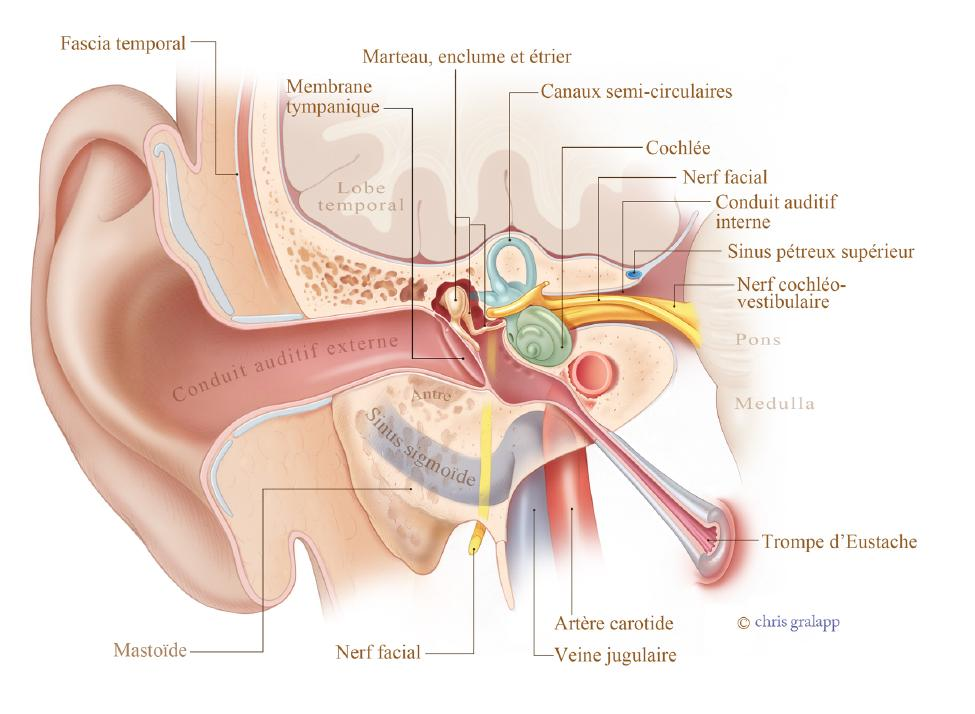
\includegraphics[width=0.7\linewidth]{images/20160624Berufsfeldgruppen.jpg}
	\caption[Titre pour toc]{Titre long pour la page}
	\label{fig:-20160624berufsfeldgruppen}
\end{figure}


%\begin{figure}
%
%\caption[Schéma global]
%%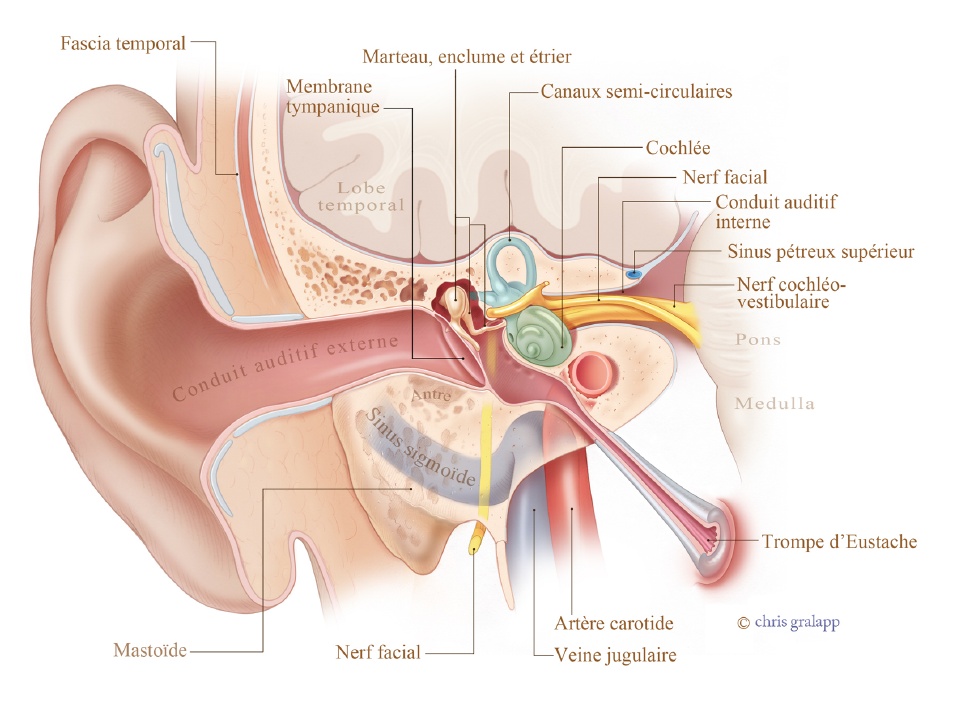
\includegraphics[scale=0.2]{images/20160624Berufsfeldgruppen.png}
%\end{figure}

\paragraph{L'oreille se situe à l'intérieur de l'un des os du crâne, le temporal,
et plus précisément la pyramide pétreuse ou rocher. Elle se compose
de trois parties : externe, moyenne, interne.}
\begin{enumerate}
\item L'oreille externe : formée du pavillon et du méat acoustique externe
(canal auditif). Les ondes sonores entrent dans le méat et percutent
une membrane de 60 mm2, appelée tympan, et la font vibrer. Cette membrane
sépare l'oreille externe de l'oreille moyenne. Selon Tomatis, elle
joue un rôle de filtre des graves et d'amplificateur des aigus.\footnote{Biologie humaine, principes d'anatomie et de physiologie, Elaine N.Marieb,
éd.Pearson Education, 8ème édition, chap. 8, pp.319-321}
\item L'oreille moyenne : se trouve dans l'os temporal constituée de petites
cavités dont une, centrale, qui est la caisse du tympan. Sa limite
médiale est une paroi osseuse percée de deux orifices , la fenêtre
du vestibule et la fenêtre de la cochlée. La trompe auditive ou d'Eustache
est un conduit oblique qui relie l'oreille moyenne à la gorge et sert
à équilibrer la pression de l'air entre l'oreille moyenne et l'extérieur.
Les trois osselets de l'ouïe sont : le marteau, l'enclume et l'étrier
( les plus petits os du corps). Ils transmettent les vibrations du
tympan aux liquides de l'oreille interne. Le marteau et l'étrier sontse
trouve dans l'os temporal constituée de petites cavités dont une,
centrale, qui est la caisse du tympan. Les trois osselets de l'ouïe
sont : le marteau, l'enclume et l'étrier ( les plus petits os du corps);
le marteau et l'étrier sont commandés chacun par un muscle. D'après
Tomatis, son rôle est double : protéger l'oreille interne des sons
trop forts et celui de cibler les sons à écouter.
\item L'oreille interne : est l' organe de l\textquoteright audition. Il
est constitué d'une coque osseuse d'une très grande densité( la plus
importante du corps), contenant un corps membraneux qui en épouse
la forme. L'oreille interne est une enfilade de cavités osseuses portant
le nom de labyrinthe osseux. Il comprend trois subdivisions : la cochlée,
le vestibule du labyrinthe et les canaux semi-circulaires. Le labyrinthe
osseux est rempli de périlymphe, un liquide. Et dans ce périlymphe
flotte le le labyrinthe membraneux qui contient lui-même un liquide
plus épais appelé endolymphe. Ils jouent leur rôle dans l'équilibre
statique et dynamique.Le vestibule et les canaux semi-circulaires
sont les organes de l\textquoteright équilibration , la cochlée ou
limaçon est l'organe de l'audition. 
\end{enumerate}
\begin{quotation}
\char`\"{}C'est le son qui a fabriqué l'oreille et si tu veux connaître
le son, apprends d'abord à étudier l\textquoteright oreille\char`\"{}.
Hermès Trimégiste
\end{quotation}

\subsection{La physiologie de l'oreille : }

Le chemin du son dans l'oreille jusqu'au cerveau : 

Chaque son parvenant à l'oreille entre dans le pavillon et se propage
dans le conduit auditif. Les vibrations de l'onde sonore mettent en
mouvement le tympan lié aux trois petits os (marteau, enclume, étrier).
La transformation (et l\textquoteright amplification) des vibrations
aériennes en vibrations solidiennes se fait par l\textquoteright intermédiaire
des osselets : les vibrations du tympan entraînent successivement
celles du bloc marteau-enclume puis celle de l\textquoteright étrier,
qui les transmet à l\textquoteright oreille interne via la fenêtre
ovale.

Le rapport de levier effectif entre le marteau et l\textquoteright enclume
(de l\textquoteright ordre de 20), d\textquoteright une part, et le
rapport de surfaces entre le tympan (60mm2) et la platine de l\textquoteright étrier
(30 mm2) d\textquoteright autre part font du système tympano-ossiculaire
un véritable amplificateur permettant à l\textquoteright énergie sonore
d\textquoteright être transmise presque intégralement à l\textquoteright oreille
interne.

A partir de 80 dB, un réflexe protecteur (stapédien) est mis en place
afin de réduire la transmission des pressions vers l\textquoteright oreille
interne, par l\textquoteright intermédiaire des osselets et des muscles
qui rattachent le marteau et l\textquoteright étrier aux parois de
la caisse du tympan. Il s'agit ainsi d' un procédé mécanique qui amplifient
les vibrations atteignant la cochlée. 
\begin{quotation}
La cochlée à son tour ``va transformer ces vibrations en impulsions
nerveuses véhiculées par le nerf auditif.'' (...)Les cellules ciliées
tapies dans la membrane cochléaire ``transforment ces vibrations
en messages électriques, circulant dans le nerf auditif. (...) Et
ces informations vont ``se diriger vers le cortex cérébral, via plusieurs
relais.(...) ``Comme certaines fibres issues de chaque oreille croisent
la ligne médiane, chaque aire auditive reçoit des signaux des deux
oreilles.'' De plus, ``tout au long du trajet, le message subit
des transformations dues aux caractéristiques de l'activité des neurones.''
Retenons que `` les cellules ciliées proches de l'étrier sont activées
par les sons aigus, et celles situées au sommet de la cochlée le sont
par les sons de basse fréquence''.(...) `` Une scène auditive est
mêlée d'un ensemble d'ondes acoustiques et son analyse se ferait non
seulement tout au long du système auditif avec des indices comme la
fréquence et l'intensité mais aussi au-delà, pour utiliser les informations
liées aux autres sens ou au contexte.'' \footnote{E.Bigand,\emph{ Le cerveau mélomane}. pp.15-16.Ed.Belin, novembre
2013}
\end{quotation}

\section{Critiques et interrogations :}

Tomatis s'oppose sur plusieurs points aux théories classiques de la
physiologie auditive : 
\begin{itemize}
\item l'oreille moyenne et son rôle de transmetteur 
\item l'analyse fréquentielle au niveau de la cochlée
\end{itemize}
Son originalité réside dans sa conception de la transmission du son
au niveau de l'oreille interne. 

Il propose une nouvelle compréhension de l'oreille, celle-ci étant,
à son regard, un organe actif dans le sens suivant :
\begin{itemize}
\item L'oreille moyenne, grâce aux muscles de l'étrier et du marteau, fait
un travail de visée en ciblant les sons à écouter : le tympan se tend
pour se mettre en résonance avec les sons à percevoir.
\item Il fait aussi un autre travail qui est celui de sélectionner des sons
pour se protéger : la tension tympanique se détend pour amortir l'intensité
sonore qui inonde l'oreille interne. 
\end{itemize}
\begin{description}
\item [{Selon}] la théorie de Georg Békésy, qui obtint le prix Nobel de
physiologie en 1961 et qui reste encore la référence classique, l'oreille
ne sert qu'à transmettre les sons de manière passive comme peut le
faire un micro. Le rôle des osselets se limite à la transmission du
son. Comme déjà décrit plus haut, les sons font vibrer le tympan qui,
étant attaché au marteau, répercute ces ondes acoustiques en mouvements
mécaniques via les osselets. L'étrier transmet ensuite ces mouvements
à l'oreille interne en jouant comme un piston au niveau de la fenêtre
ovale. L'information acoustique est alors transmise sous forme d'ondes
liquidiennes ou encore de tourbillons. Les tourbillons sont analysés(
amplitude et vitesse) en termes de fréquences et de volume par les
cellules ciliées qui tapissent l'oreille interne. 
\item [{Selon}] Tomatis, cette théorie a de nombreuses incohérences. L'une
d'entr' elles serait que cette démonstration ne marche qu'avec un
son pur \footnote{un son pur est constitué d'une unique fréquence ou onde}.
Or, les sons purs n'existent pas dans la nature, car ils sont, au
contraire, complexes et formés d'une multitude de fréquences et d'intensités
variées. Et cette complexité ne peut pas être transmise sans perte
et instantanément par des mouvements mécaniques et retransformée en
tourbillons. De plus, il y a un espace entre l'enclume et l'étrier,
microscopique à l'oeil nu mais énorme sur un plan comparatif, c'est
un hiatus considérable à l'échelle atomique puisqu'il est de l'ordre
d'un millimètre. Ce phénomène reste inexpliquable sur le plan de la
physique pure.
\end{description}
\footnote{Conférence au IIème Congrès International d'Audio-Psycho-Phonologie
Paris 1972 \emph{: Nouvelles théories sur la physiologie auditive}} : il est de l'ordre de s'interroger s'il est possible que la transmission
puisse se faire dans ces conditions. On peut imaginer que le son passe
partout, par les ligaments de jonction des osselets ou les espaces
inter-ossiculaires mais

ce n'était pas scientifiquement prouvable lors d'une de ses conférences
en 1972. Peut-être l'est-il à l'heure actuelle, mais nous n'en avons
pas trouvé trace. 

Nous allons aborder la conduction osseuse qui pourrait nous aider
dans cette compréhension.
\begin{description}
\item [{La}] conduction osseuse : lorsque l'on fait l'expérience de se
boucher les oreilles et de parler normalement, on se rend compte que
notre voix se propage principalement par les os de la tête. Comment
expliquer que l'on perçoive parfaitement bien les sons par conduction
osseuse en mettant un vibrateur conducteur de son sur la boîte crânienne
? et ce, même si l'oreille moyenne est abîmée ( tympan percé, osselets
non fonctionnels) . Selon une dernière recherche, effectivement, le
son stimule l'oreille de deux manières : par voie aérienne en transitant
par les trois parties de l'oreille et par voie osseuse en stimulant
directement l'oreille interne par vibrations des structures osseuses
qui l'entourent. Ce site : oreillemudry.ch a été mis à jour le 28.07.2016.
Il relève l'importance de la voie osseuse mais ne signale aucun nouvel
élément dans la transmission fréquentielle que celle dite classique,
évoquée plus haut. 
\item [{Schéma:}] Physiologie de l\textquoteright audition 
\item [{D'après}] Tomatis, les sons arrivent bien par le canal auditif
jusqu'au tympan. L'onde acoustique excite la membrane tympanique et
par voie de conséquence, l'os de la caisse du tympan. A l'instar d'une
peau de tambour qui fait chanter le bois auquel elle est attachée,
c'est toute la boîte crânienne qui inondée de sons et en particulier
l'oreille interne. Celle-ci, de par sa grande densité, capte les sons
et résonne comme du cristal. (\marginpar{ La transmission du son par l'os est de 5000 m/s.}
Les fréquences qui forment les sons vont ainsi exciter les cellules
ciliées qui tapissent la cochlée, tel un piano enroulé. 
\item [{Avec}] sa théorie, l'analyse multifréquentielle ne se pose plus
: chaque fréquence se dirige instantanément et naturellement\emph{
}vers la cellule ciliée qui lui correspond. C'est grâce à la forme
particulière\emph{ }du limaçon qu'il y a un tri fréquentiel instantané.
Le son identique fréquentiellement s'installe toujours au même endroit
, sur une ligne isofréquentielle, qui est une tranche perpendiculaire
à l'axe.
\end{description}
Et le phénomène des tourbillons n'a donc pas pour fonction de transmettre
les sons mais interviennent pour déclencher les mécanismes d'adaptation
aux bruits. 
\begin{description}
\item [{Comment}] cela se passse-t-il ? Lorsque l'intensité des sons augmente,
l'excitation des cellules ciliées provoque des perturbations liquidiennes
dans l'oreille interne, c.à.dire des tourbillons. Ceux-ci se propagent
et sont amortis par l'étrier. Si les sons atteignent une intensité
dangeureuse pour les cellules ciliées, l'étrier réagit fortement et
entraîne une réaction du marteau qui modifie la tension du tympan.
A son tour, le tympan, relâché, amortit le volume sonore transmis
à l'oreille interne, comme la paupière qui se ferme quand la lumière
est trop intense.
\end{description}

\subparagraph*{``Le tympan se met dans un certain état de tension pour jouer le
rôle d\textquoteright un diapason qui fait vibrer toute la boîte cranienne
par l'intermédiaire du sulcus tympani. \emph{C'est toute la boîte
crânienne qui vibre et qui transmet le son à la vésicule labyrinthique
et non à la chaîne ossiculaire que l'on a l'habitude de considérer
comme le véhicule du son. }La chaîne ossiculaire est un ensemble qui
joue le rôle d'adapteur, de régulateur et non de transmetteur. La
conduction du son par l\textquoteright air puis par l'os doit donc
être étudiée d\textquoteright une façon complémentaire afin que l'on
puisse déterminer par la suite la posture d'écoute du sujet.''\protect\footnote{key 14, Entretien réalisé par B.Auriol avec Tomatis, Anvers 1973}}

Il serait passionnant de faire une étude comparative approfondie des
recherches actuelles au sujet de la physiologie auditive. Génère-t-elle
toujours autant d' interrogations et de débats ?

Christine Petit note et relève par ces recherches le rôle important
et indéniable de la cochlée sur notre audition et spécifie qu'encore
à l'heure actuelle, il reste très mystérieux. \nomenclature{cochlée}{Anatomie : organe de l'audition,appareil sensoriel, en forme de spirale, la cochlée, incluse dans l'os du rocher, forme le limaçon membraneux ,se situe dans l'oreille interne et permet de déceler des sons extrêmement faibles, de discréminer des fréquences et de masquer des sons faibles par des sons forts. }
''C'est une sorte de minuscule appareil électroacoustique capable
de discréminer des sons extrêmement faibles, capable de \emph{masquer
les sons faibles par des sons forts}, pouvant \emph{distordre les
sons,} et en conséquent, \emph{capable d'élaborer un traitement extrêmement
sophistiqué des sons}.''

\footnote{ Christine Petit, titulaire de la chaire Génétique et physiologie
cellulaire au Collège de France, entretien en novembre 2012, réalisé
par Laurent Salters et Vincent Gaullier, Look at science : le système
sensoriel auditif confirme lors d'un entretien réalisé en 2012 le
rôle indéniable de la cochlée. key-13}
\begin{description}
\item [{Observation}] et critiques sur l'application et l'utilisation de
la méthode Tomatis : 
\item [{C'est}] une méthode controversée car il manque des études médicales
de grande envergure sur le sujet, susceptibles d'une évaluation statistique
sûre. Selon Pierre Lane, journaliste de l'émission Envoyé spécial
\footnote{Emission télévisée ``Envoyé spécial''16.5.1991}, Tomatis
a inventé une méthode qui est très critiquée mais qui a donné des
résultats. Elle ouvre l'oreille par des procédés mécaniques pour atteindre
des domaines spécialisés , que ce soit en médecine, en psychologie,
en ostéopathie, etc. Pierre Lane précise qu'il s'agit d'un outil proposé
en complément de leur pratique à de nombreux spécialistes. 
\item [{Au}] fil des années, de nombreuses études scientifques et cliniques
ont été faites. Il est possible d'en trouver le contenu sur le site
internet officiel Tomatis : Tomatis Research and Publication des plus
anciens aux plus récents en 2016.\footnote{www.tomatisassociation.org}
Nous pouvons citer les travaux des Docteur Du Plessis sur l'effet
Tomatis sur l'anxiété en milieu scolaire et universitaire,\footnote{Troubles psychologiques : Etude du Plessis (Université de Potchefstroon
- Afrique du Sud)avec un comparatif Pre / Post niveau d\textquoteright anxiété.
Du Plessis a étudié le cas de 29 étudiants sujets à l\textquoteright anxiété.
10 étudiants ont suivi des séances d\textquoteright écoute Tomatis\textregistered ,
9 ont suivi une psychothérapie classique et 10 ont été choisis pour
former le groupe contrôle. Le groupe Tomatis\textregistered{} a montré
une réduction significative de l\textquoteright anxiété, tandis que
les resultats sont mitigés pour ceux qui ont suivi une psychothérapie
et inexistants pour le groupe contrôle.

Une seconde étude De Plessis a démontré qu\textquoteright après 14,3
mois le niveau d\textquoteright anxiété avait continué à baisser fortement
pour le groupe Tomatis\textregistered{} alors qu\textquoteright aucun
changement n\textquoteright apparaissait pour le groupe contrôle.} \footnote{Du Plessis W.F. and Van Jaarsveld, P.E.(1988), \emph{Audio-psycho-phonology
: A comparative outcome study on anxious primary school pupils, }S\emph{.}Afr.
Tydskr.Sielk.1988,18(4)144-151;

Du Plessis,W.F., Burger,S.(2001)(..) \emph{A pilot study involving
the Tomatis method.}Sud Africa J.Psychol. et plus récemment encore
(2004) \emph{The Impact of a Combined Tomatis and Psycho-Educational
Program on Weight Preoccupied, Female south African Students, }International
Journal of Tomatis Method Research,1(1)54-65} les travaux de Jan Gerritsen, PhD (2009) \footnote{\emph{A Review of Research done on Tomatis Auditory Stimulation}},
les études du dr.P.E.Van Jaarsveld, psychologue à l'Université de
Potchefstroom en Afrique du Sud sur l'action de l'audio-psycho-phonologie
sur le bégaiement \footnote{\emph{The Effect of Audio-Psycho-Phonology on Stuttering}}.
\item [{Plus}] récemment nous citerons encore en dernier lieu la parution
de la dernière recherche menée en collaboration avec le CNRS. Cette
recherche a été publiée dans la revue scientifique \char`\"{}Journal
of Affective Disorders\char`\"{}. Elle a donc fait l'objet d'une validation
par un comité de lecture scientifique. Elle démontre qu'il existe
un lien important et certain entre la difficulté à percevoir certains
sons et l'existence de troubles émotionnels. L'intérêt de stimuler
le cerveau en lui permettant de capter plus facilement ces sons est
donc dès lors évident. Il s'agit d'une étude pilote du Dr.Carlos Escera
de l'Université de Barcelone en 2014 \footnote{\begin{description}
\item [{\emph{http://tomatisassociation.org/scientific-validation-of-the-tomatis-effect-eeg-recordings-of-sound-from-brainstem-to-cerebral-cortex-encoding-university-of-barcelona-2014/}}]~
\end{description}
}sur l'effet d'une technique particulière employée avec l'Oreille Electronique
-la bascule électronique \footnote{( qui permet de créer une alternance entre deux conditions perceptives
du même message sonore -passage soudain et imprévu de fréquences graves
à des fréquences aigues) . }
\item [{Nous}]~
\end{description}
\emph{}\footnote{\emph{``Les seuils auditifis des sons purs sont diminués chez les
personnes déprimées avec des troubles de stress post-traumatique.''}
\begin{description}
\item [{\emph{\char`\"{}Pure-tone}}] \emph{auditory thresholds are decreased
in depressed people with post-traumatic stress disorder\char`\"{}
Journal of Affective disorders.} Recherche du CNRS en collaboration
avec Tomatis Developpement S.A.
\end{description}
Auteurs : Stéphanie Aubert-Khalfa; Emmanuelle Reynaud; Myriam El Khoury;
Olivier Blin - INCM, UMR CNRS 6193, Jean-Pierre Granier - TOMATIS
DEVELOPPEMENT S.A. Eva-Maria Grosse; Jean-Claude Samuelian - Pôle
Psychiatrie Centre, La Conception Hospital }

Il y a lieu d'observer et de remarquer que certaines de ces études
ont été menées en collaboration avec la société Tomatis actuelle,
ce qui enlève quelque peu l'intégrité de la recherche.
\begin{quotation}
Selon le Dr.med.Inge Flehming\footnote{Dr.med.Inge Flehming, neurologue, neuropédiatre, texte publié en allemand
en 1996,\emph{``Grundsatz-Gutachten zur Behandlungsmethode nach Prof.Tomatis''http://www.analytische-hoertherapie.de/uploads/tx\_templavoila/Grundsatzgutachten\_zur\_Behandlungsmethode\_nach\_Prof.\_Tomatis.pdf}}''il est compréhensible que les médecins ORL n'en soient pas convaincus
par le fait que les objectifs thérapeutiques sont différents. L'ORL
cherche à améliorer l'audition tandis que le neurologue ou le neuropédiatre
ne s'en préoccupe pas, mais cherche à comprendre les raisons pour
lesquelles certains sujets ont des difficultés à appréhender ce qu'ils
entendent, c'est-à-dire à traiter correctement l'information au niveau
du cerveau.''
\end{quotation}
\begin{quote}
\footnote{``Or le traitement central correct d'un stimulus relayé au cerveau
par les voies sensorielles présuppose l'acquisition d'une synergie
parfaite entre les systèmes sensoriels au niveau de l'organe central
(le cerveau), un processus nommé \char`\"{}intégration sensorielle\char`\"{}.
Dans ce contexte, Tomatis distingue entre \char`\"{}l'audition\char`\"{},
prise comme l'expression de la réalisation acoustique de l'impulsion
auditive dans le cerveau, et \char`\"{}l'écoute\char`\"{}, prise comme
un processus \char`\"{}d'écoute consciente\char`\"{}, impliquant l'attention
immédiate et la conscience subjective de l'individu. En présence d'une
stimulation adéquate, toutes les voies sensorielles du corps sont
en mesure de réaliser l'intégration sensorielle, prise comme synergie
des systèmes sensoriels, et leur interconnexion au niveau du cerveau.
L'oreille joue néanmoins un rôle tout à fait particulier dans ce processus.
En effet, le labyrinthe osseux de l'oreille interne réunit deux systèmes
sensoriels diamétralement opposés, mais néanmoins fondamentaux, l'un
et l'autre, dans un espace très réduit. Le système auditif est le
premier système sensoriel achevé sur le plan anatomique dans l'évolution
prénatale de l'enfant. Cela veut dire que dès une phase précoce de
la grossesse, l'audition est entièrement opérationnelle, et mise à
contribution. De nos jours, nous savons que la formation de synapses
entre les neurones du cerveau, c'est-à-dire le câblage et l'interconnexion
des milliards de neurones présents dans le cerveau, obéit à un processus
activement contrôlé, où des dendrites \char`\"{}chercheurs\char`\"{}
et des dendrites \char`\"{}récepteurs\char`\"{}, guidés en-cela par
des molécules dits \char`\"{}neuro-tactiques\char`\"{}, établissent
des liens persistants avec une précision tout à fait remarquable.
Ces liens, qui sont d'une importance vitale pour l'individu, resteront
pour la plupart en place pendant toute sa vie. Ce processus de formation
de synapses ou d'interconnexion des neurones débute chez l'enfant
dès les premières semaines de la grossesse. Il est d'ailleurs stimulé
par la sollicitation active des organes sensoriels. Dans ce contexte,
et à juste titre, Tomatis souligne l'importance du développement sensoriel
prénatal de l'enfant. Il affirme que l'audition précoce, intra-utérine
de l'enfant, joue un rôle moteur pour le développement de tous les
systèmes sensoriels de ce dernier, leur permettant de fonctionner
en synergie, de former un réseau de connexions cérébrales dès un âge
précoce, à savoir longtemps avant la naissance, favorisant ainsi la
maturation du cerveau dans son ensemble.''(...)L'influence réciproque
entre les systèmes auditif et vestibulaire ne se limite pas à la proximité
spatiale des deux organes dans l'oreille interne. En effet, il y a
des connexions centralisées au niveau du cerveau entre le nerf acoustique
et d'autres facultés sensorielles, qui touchent bien évidemment aussi
l'organe de l'équilibre. (résultat de frayeur et réaction de fuite
dûe à un bruit : un enchaînement de réflexes liés à la fois à la proprioception
et au système vestibulaire. C'est tout le corps qui réagit en esquissant
une réaction de fuite.'' (...)}
\end{quote}
\begin{quotation}
(...)``La thérapie selon Tomatis, en ce qu'elle influence les mécanismes
de la perception auditive, a un effet bénéfique global, holistique,
qui n'opère pas tant sur l'audition que sur l'écoute attentive, la
régulation de la tonicité musculaire, la coordination entre la motricité
globale et la motricité fine, et l'érection de l'individu dans l'espace.
Bien évidemment, ce sont des aspects auxquels les neurologues du développement
ou neuropédiatres sont plus sensibles que les ORL, dont les objectifs
s'inscrivent dans un tout autre domaine. La thérapie selon Tomatis
ne relève pas de la médecine alternative, ni de l'ésotérisme, mais
d'une neurophysiologie appliquée et holistique ; à ce titre, elle
joue un rôle tout à fait marquant.''\footnote{Dr.med. Inge Flemming}
\end{quotation}
Force nous est de constater que cette même forme de controverse existe
aussi avec d'autres types de thérapies telle l'acupuncture, bien qu'ancestrale
et riche de résultats : les mécanismes en jeu étant non élucidés et
les études d'évaluation encore insuffisantes. 

La neuroscience nous apporte beaucoup dans le domaine du cerveau et
de la musique. Rien n'est encore élucidé. Peut-être ces recherches
aboutiront-elles avec des résultats qui prouveront cette méthode ou
la démonteront ? Pour l'instant, sans preuve scientifique à l'appui,
nous continuons à investiguer dans les critiques.

D'autre part, comme pour tous types de thérapies, la qualité de prise
en charge varie également avec la qualité du médecin ou du thérapeute.
Ceux-ci ne sont pas forcément à la hauteur des attentes du patient
qui doit toujours garder un esprit critique.

Un des reproches tout à fait justifié de la méthode Tomatis est parfois
le manque de suivi. Le patient se trouve un peu ``largué'', avec
une oreille remise au point mais avec laquelle il se sent perdu. Il
faut du temps pour qu'il puisse s'y habituer et que les nouvelles
façons de fonctionner s'intègrent. L'accompagnement du patient dans
la phase active nécessite du temps. L' investissement est différent.
Nous rentrons de plein fouet dans le domaine de compétences des champs
d'application des thérapeutes.Ce peut être celui des logopédistes
par exemple, ou des musicothérapeutes.

\section{Technique de travail sous ``Oreille électronique'' :}

Dès 1952, comme preuve et application des trois lois qu'il avait énoncées,
Tomatis a concentré ses efforts de recherche sur la mise au point
d'un appareil susceptible de mondifier la manière d'entendre et, par
voie de conséquence, la façon de parler d'un sujet. Par cet appareil,
le but était d'obliger l'oreille à utiliser un mode d'accomodation
déterminant une manière d'entendre typique et entraînant le geste
vocal correspondant.

Conçue déjà en 1947, L'Oreille Electronique est ``la réplique parfaite
d'une oreille humaine'' nous dit son inventeur. L'oreille parfaite
saurait écouter ; elle passe de l'entendre à écouter, elle se tend
vers l'information qui lui arrive. Ce n'est pas si facile, ce n'est
pas inné. Et si on met l'Oreille électronique en parallèle avec une
oreille qui ne rentre pas dans cette dynamique, elle va l'entraîner.
Elle sert à faire faire une gymnastique bien précise ou un jeu de
contractions.

L'adaptation de l'oreille moyenne se fait par le jeu des contractions
du muscle du marteau et du muscle de l'étrier.
\begin{itemize}
\item Le muscle du marteau agit sur la convexité imposée au tympan, qui
se comporte alors comme une lentille acoustique, sorte de cristallin
auditif.
\item Le muscle de l'étrier régule le jeu de l'oreille interne, qui sait,
à la manière d'un prisme, étaler la gamme des sons en spectre acoustique.
\end{itemize}
Cette accomodation plus ou moins rapide, plus ou moins complexe, permet
d'ouvrir telle ou telle bande passante auditive, d'agrandir selon
les besoins, le diaphragme d'ouverture.

L'Oreille Electronique impose ce jeu à l'oreille.

ll y aura un travail dit ``passif'' dans le sens que ce sera d'abord
un travail d' écoute de musiques et un travail dit ``actif'' où
la personne s'implique directement en émettant des sons avec la possibité
de travailler et d'être corrigé immédiatement sous Oreille Electronique.

Dans le but de faire faire cette gymnastique microscopique aux muscles
de l'oreille, ces musiques peuvent être préparées avec un jeu de bascule{*}(
cf explication 3.3.3.) qui alterne le passage des basses aux hautes
fréquences; elles peuvent aussi l'être avec un certain pourcentage
de filtrages \footnote{}qui va varier et s'ajuster selon la personne
et le résultat des tests d'écoute. Pour stimuler le désir d'écoute
du patient, il est aussi possible de préparer des musiques avec une
technique particulière, dénommée retard, agissant sur le muscle de
l'étrier, c'est-à-dire sur la conduction osseuse. Une autre technique
est celle de la précession, qui aidera à viser et décoder les messages,
en agissant sur le tympan, c'est-à-dire sur la conduction aérienne. 

Ce type de traitement n'est donc pas le fruit du hasard mais d'une
longue recherche pour la mise au point de ces différentes techniques
sous Oreille Electronique.

\section{Travail ``passif'' et ``actif''sous Oreille Electronique}

\subsection{Technique dans le travail passif et actif : }
\begin{itemize}
\item La façon générale de procéder est l'alternance d'écoute de musiques,
de travail actif avec la voix, de tests d'écoute, de pauses.
\end{itemize}
Avant les séances : un test d'écoute, focus sur l'audition avec un
graphique.

Après les séances : le même test, avec visualisation d' une évolution
ou d'une transformation de l'écoute du patient : un changement sera
visible ou ne le sera pas.

\subparagraph{Dans le travail passif : }
\begin{description}
\item [{1\textdegree Session}] de 25 à 30h d'écoute : le patient écoute
deux heures de musique par jour pendant 13 à 15 jours consécutifs;
un deuxième test à la fin de ce travail; ensuite, une pause pendant
4 à 6 semaines.
\item [{2\textdegree Session}] de 25 à 30h d'écoute : 3ème Test, à nouveau
deux heures d'écoute pendant 13 jours à 15 jours; puis 4ème test,
suivi d'une pause d'une durée de 4 à 8 semaines.
\item [{3\textdegree Session}] : la même façon de procéder que les deux
autres. 
\end{description}
Le choix et le traitement des musiques peuvent être très différents
selon le patient et sa pathologie.

But du travail passif : \emph{``}Ouverture\emph{'' }de l'oreille
aux sons : sensibiliser à certains sons avec l'objectif de réintégrer
des fréquences perdues ou annihilées inconsciemment ou volontairement. 

Cette technique de travail se sert du son pour provoquer un résultat
physiologique. Elle dérange les habitudes d'écoute pour faire agir
et ré-agir le patient. Cette phase est parfois totalement rejetée
par le patient.

\subparagraph{Dans le travail actif :}

Après avoir été stimulé et ouvert aux sons environnants, le patient
est amené par le thérapeute à travailler sa voix. On cible un travail
actif de la voix à l'aide des écouteurs spécifiques de la méthode
car la correction de la voix y est instantanée et instaure les bons
réflexes de la boucle audio-vocale. C'est un processus naturel par
lequel l'individu assimile et analyse l'information sonore qu'il reçoit
et ajuste en retour l'information sonore qu'il émet. Le patient va
commencer à s'en servir ``à volonté'', c'est-à-dire d'ajuster et
d'analyser ce va-et-vient permanent entre l'écoute et l'émission vocale
afin de créer une forme de réflexes sur lesquels il peut ``s'asseoir''. 

Cette phase de la thérapie est importante et parfois très délicate
pour le patient. Accepter d'entendre sa propre voix n'est pas toujours
simple et l'encadrement et le soutien sont nécessaires pour permettre
au patient de franchir cette étape. Lorsqu'elle se passe bien , il
y a en quelque sorte réintégration de la voix dans le corps. Le patient
apprend à créer lui-même cette boucle phonatoire sur laquelle il va
pouvoir se reposer, se ressourcer, se régénérer pour être totalement
autonome au bout de sa restructuration : une reprise en main qui va
lui permettre d'``être et de se sentir auteur de sa propre vie''. 

\subparagraph{\textmd{\emph{``L'émission vocale confirme et reconfirme à chaque
fois le sujet dans son intégrité et son identité.''A.Tomatis}}}

\footnote{Tomatis en fait une description précise dans la troisième partie de
son livre\emph{ L'oreille et la voix, pp.185-301}}

Vu et décrit sous un oeil scientifique, ``il existe une interaction
constante entre le traitement auditif et le traitement moteur de la
voix, entre l'information sensorielle et les programmes moteurs impliqués
dans la parole ou le chant. Le programme moteur qui a été déclenché
pour la parole permet au cerveau de faire des hypothèses constantes
sur les conséquences acoustiques du geste vocal qui est sur le point
d'être réalisé. Ensuite, l'hypothèse est comparée à l'information
auditive reçue. C'est principalement à travers l'activation de la
boucle audio-vocale que peu à peu, le cerveau va modifier l'hypothèse
qu'il a construite à propos des conséquences acoustiques du geste
vocal sur le point d'être réalisé.'' \footnote{J.P.Granier, Tomatis Développement,\emph{ Conférence Paris}, 13.5.2012}

\chapter{La musicothérapie et la psychothérapie}

Nous savons que la musicothérqpie est de plus en plus intégrée dans
les milieux psychiatriques.  Comme il s'agit du domaine dans lequel je
travaille et que j'ai choisi d'analyser pour ce travail, nous
aimerions traiter plus précisément des sujets de la dépression et du
burn-out, très souvent associés.


\chapter{La dépression}


\chapter{Le test Tomatis : }

\section{Explication :}

Tomatis a mis au point un test spécifique destiné à fournir une traduction
graphique de l'écoute.

Ce test est fait pour :
\begin{itemize}
\item constater la posture d'écoute de la personne ainsi que l'articulation
des trois systèmes : la fonction de dynamisation, la fonction vestibulaire,
et la fonction d'écoute.
\item observer les modifications et les évolutions des courbes au cours
de la thérapie.
\end{itemize}
Tomatis était un médecin O.R.L, un clinicien et  ses constatations
sont issues d'observations ; il a commencé en faisant
des tests d'écoute dénommés audiogramme, avec des résultats concernant  des pertes auditives, des troubles de l'oreille
comme le scotome, lésion pathognomonique (qui est le terme spécifique
d'une maladie en médecine). 

En 1947, il dirigeait le Laboratoire d'acoustique
des arsenaux de l'aéronotique et devait examiner avec l'audiogramme l'audition détériorée
des personnes travaillant sur les bancs d'essais des réacteurs supersoniques.Tomatis constata que les pertes auditives étaient accompagnées non seulement  d'une
déformation assez nette de la voix mais aussi de troubles cognitifs, de trouble du comportement ou d'une modification de la posture. Avec
un chanteur venu pour un problème dans un  registre de voix il releva une lésion de l'oreille similaire
à celles observées chez les ouvriers des arsenaux. En fait, ce chanteur
souffrait de surdité professionnelle. Il commença alors à approfondir
ce parallélisme constant entre l'examen audiométrique et la courbe
d'enveloppe de l'analyse des fréquences de la voix Il était totalement
inutile de soigner ce chanteur avec de la sulfate de
strychnine, selon les prescriptions habituelles des phoniatres de
l'époque. Aucun résultat n'était obtenu en tendant les cordes vocales
comme un violon qu'on accorde. Il émit alors l'hypothèse fondatrice
que la perturbation de la voix n'était pas due à un défaut des cordes
vocales mais à une détérioration de l'oreille. . Puis il eut l'idée
d'essayer de corriger la voix défectueuse en imposant à l'oreille
une courbe de réponse auditive idéale. Pour réaliser cette stimulation
de l'oreille, il mit au point un appareil électronique appelé Oreille
Electronique ou appareil à ``effet Tomatis''. Et, dès les premières
séances, il constata une amélioration temporaire de la voix qui devint
peu à peu permanente avec de l'entraînement. Il avait fait ce lien épatant entre la difficulté d'entendre et celle d'émettre.

Tomatis a défini la «courbe d\textquoteright écoute idéale» après
bien de nombreuses expériences sur des personnes qui souffraient de
problèmes de perception auditive. Elle correspond à l'oreille absolue
des chanteurs et des musiciens. Tomatis étudia le ténor italien Enrico
Caruso (1873-1921) dont il analysa la voix à partir des enregistrements
de ses vocalises sur vinyles. Caruso représentait la courbe auditive
optimale. Il décida de se référer à  sa voix pour élaborer la courbe idéale surnommée «courbe de Caruso».

Sur le plan de la physique pure, elle indique les réponses de l'oreille
lorsque celle-ci fonctionne bien. Elle répond en fait à la courbe
de Wegel dite \char`\"{}courbe en citron\char`\"{}, inversée.\footnote{
		"Effectivement la courbe de Wegel est la courbe de réponse obtenue
lorsque sont posées en abscisses les fréquences, et en ordonnées ascendantes
les intensités. Un premier seuil s'obtient, en partie basse, suivant
un minimum qui commence dans les fréquences graves à environ 40-50
dB, avoisine ensuite la courbe des abscisses entre 2000 et 3000 Hz
et redevient ascendante à 40 / 50 dBs dans les aigus entre 8 000 et
10 000 Hz. Cette courbe se complète et prend l'allure de citron selon
l'expression qu'on lui confère lorsqu\textquoteright on envoie des
sons d'intensité croissante et qu'on obtient alors une courbe des
seuils maxima qui se déterminent là où l'oreille commence à souffrir,
d'où le nom de \char`\"{}seuil de la douleur\char`\"{}.Ces seuils
commencent dans les graves, également à 50-60 dB rejoignant la première
courbe, puis ils atteignent 120 à 130 dB entre 2000 et 3000 Hz pour
chuter ensuite dans les aigus en rejoignant également la première
courbe. La ligne médiane qui se situe aux environs de 50-60 dBs, qui
est linéaire représente une zone dite \char`\"{}Zone de Munsen''.
Elle répond à la dynamique de l\textquoteright oreille, c\textquoteright est
à dire à sa zone \char`\"{}optimale\char`\"{} de fonctionnement sans
distorsion. Dans toutes les autres zones, l\textquoteright oreille
agit comme un filtre dont les pentes sont variables en fonction de
l\textquoteright intensité, avec un lieu de rotation situé entre 1000
et 2000 Hz. Pour pallier ces distorsions toujours difficiles à intégrer
dans la lecture des schémas, les Américains ont standardisé les audiogrammes
du type de ceux que nous utilisons tous en inversant l\textquoteright image
de Wegel et en redressant les minima pour obtenir une ligne droite.
Ces normes gardent néanmoins une zone préférentielle entre 1000 et
2000 Hz malgré les compensations de 30 à 40 dB accordées sur la courbe,
dans les graves et les aigus." Bernard Auriol, conversation, conférence.}.

L'acquisition de cette courbe idéale correspond à l\textquoteright harmonisation
du jeu de deux muscles de l\textquoteright oreille moyenne. Ce jeu
permet de régler en permanence la pression interne de la vésicule
labyrinthique en faisant intervenir les phénomènes de moindre impédance.
\footnote{Définition de l\textquoteright impédance : L'impédance acoustique
caractérise la résistance qu'un milieu oppose à sa mise en mouvement
lorsqu'il est traversé par une onde acoustique. Elle est définie comme
le rapport de la pression acoustique sur la vitesse de déplacement
locale dans un milieu, et est généralement notée Z. Elle dépend de
la température. L'impédance caractéristique d'un milieu (solide, liquide
ou gazeux) est définie comme le rapport de la pression acoustique
sur la vitesse de déplacement en milieu ouvert (c\textquoteright est-à-dire
en l'absence d'ondes réfléchies). L'impédance caractéristique est
une propriété du matériau considéré égale, dans le cas d'un espace
illimité, au produit de la masse volumique du matériau \textgreek{r}
par la vitesse du son c dans ce même matériau : Z = \textgreek{r}
. c

{[}Unités : \textgreek{r} étant exprimé en kg/m3, c en m/s, Z est
exprimé en Pa.s/m.{]} Lorsqu'une onde acoustique rencontre l'interface
séparant deux milieux d'impédances acoustiques différents, une partie
de l'onde est transmise dans l'autre milieu tandis qu'une autre partie
se réfléchit sur l'interface. On cherchera à estimer les quantités
d'énergie acoustique transmises et réfléchies.

Les ondes incidentes ( f1 ) sont transmises pour une part au second
milieu ( f2 ) et pour une autre part, elles sont réfléchies à l\textquoteright interface
entre le premier et le deuxième milieu jaune ( g1 ) (modifié d\textquoteright après
Wikipedia, 9 février 2009) }

L\textquoteright audiogramme classique donne une courbe déterminée
mais n\textquoteright indique pas pour autant si l'individu examiné
sait vraiment se servir de cette courbe pour communiquer avec les
autres au travers de son autocontrôle.

Son test permet justement de connaître l'utilisation que sait faire
un sujet de son audition.Un oeil anatomiquement parfait ne permettra
pas de déceler si le sujet sait s'en servir en visant au fusil ou
en faisant de la peinture. Toutes les nuances de couleurs qui permettent
au peintre de s'exprimer ne sont pas celles que tout un chacun voit.\footnote{Conférence, Anvers,1973.}
``L'écoute est à l\textquoteright oreille ce que la vision est à
l'½il.'' Il existe donc ``une dimension de gnosie qui apporte une
donnée complémentaire,(...) une dimension d'attention, d\textquoteright adhésion
qui s'institue dans l'écoute, prise de conscience qui s\textquoteright imbrique
à l'audition elle-même.'' 
\begin{quotation}
``Lorsque l'interprétation mentale des informations sensorielles
transmises par l'oreille est erronée, l'écoute est perturbée.''\footnote{\emph{source site officiel Tomatis.com}}
\end{quotation}
Il s'agit de distorsions d'écoute. Cette distorsion est liée au dysfonctionnement
des deux muscles de l'oreile moyenne. Leur rôle est de permettre l'arrivée
harmonieuse du son dans l'oreille interne, puis au cerveau. Car, lorsque
le message sensoriel est altéré, le cerveau se protège en déclenchant
des mécanismes d'inhibition de l'écoute.'' Tout enfant peut naître
avec ce potentiel mais celui-ci s' altére parfois avec les difficultés
de la vie. Il se ferme au monde de l'écoute et il introduit des distorsions
pour se défendre contre les agressions du monde extérieur. 

Sur le plan du test d\textquoteright écoute,\emph{ }on remarquera
alors des distorsions, des manques\emph{ }par rapport à la courbe
idéale qui se trouve sous-jacente dans tout individu. 
\begin{quotation}
``La présence d'une \emph{pente ascendante} est nécessaire pour que
l'oreille puisse bloquer les fréquences graves, les atténuer, afin
que la partie proximale de la cochlée soit utilisée, plus particulièrement
dans la zone consacrée au langage. Ceci est spécifique de l'oreille
humaine. Les auditions de certains animaux sont quant aux bandes passantes,
beaucoup plus développées que la nôtre : le dauphin, par exemple,
entend jusqu\textquoteright à 200.000 Hz, certaines chauve-souris,
certains vampires jusqu'à 150.000 Hz ; un chien entend jusqu'à 45.000
Hz. Mais ce sont là des performances qui représentent peu de chose
par rapport à la faculté qu'a l'oreille humaine d\textquoteright entendre
le langage. Et cette partie d'analyse fine exige qu'elle ne soit pas
gênée par la perception des fréquences graves. (...)''\footnote{\emph{Entretien de Tomatis par Auriol,} Anvers 1973}
\end{quotation}
\begin{quote}
\emph{``L'oreille a un psychisme.''} 
L'intégration de l'audio-thérapie et/ou de la musicothérapie a tout son sens dans le contexte ou le milieu psychiatrique. Tomatis, à notre sens, ne pouvait faire meilleure boutade
\end{quote}
De cette phrase, qui peut paraître exagérée,
nous laisse interrogatifs sur la récente parution d'un
article d'une étude franco-américaine scientifique \footnote{\emph{Etude scientifique menée au CNRS par l'acousticienne Claudia
Fritz de l'Institut Pierre et Marie Curie,}https://lejournal.cnrs.fr/diaporamas/stradivarius-la-fin-dun-mythe} au sujet des Stradivarius : elle semble ne pas lui donner totalement
tort et même l'atteste d'une autre manière : nous transformons l'écoute
selon nos attentes. Faite avec un protocole d'écoutes en aveugle avec
des violonistes professionnels et en parallèle avec un public (caché
derrière un rideau), cette étude démontre que le mythe de la suprématie
de ces instruments extrêmement chers est tombé au profit d'instruments
neufs. L'étude prouve que le cerveau transforme les informations reçues
selon les attentes que l'on a. Le rôle du cerveau dans notre perceptions
est extrêmement fort et cette étude le prouve scientifiquement. \footnote{http://www.lemonde.fr/culture/article/2014/04/10/le-stradivarius-detrone-par-les-violons-modernes\_4398681\_3246.html }

\footnote{Patrick Dumas de la Roque \emph{``L'écoute, c'est la vie''}p.43.Ed.
Jouvence, collection Trois Fontaines}

\section{Description de la passation du test d'écoute :}

Pour effectuer ce test, un appareil contenant un générateur de fréquences
appelé \char`\"{}Hearing Test\char`\"{}, émet des sons purs s'étalant
de 125 à 8000 hertz, d'octave en octave, en passant par les valeurs
1500 hertz, 3000 et 6000 hertz, et dont l'intensité, peut varier de
5 en 5 dB, de 10 à + 100 dB.. 

Ce test a pour but de déterminer les 4 paramètres suivants : 
\begin{itemize}
\item a) Recherche des seuils :
\end{itemize}
Il s'agit de rechercher d'une part les seuils d\textquoteright audibilité
minima : il est demandé au sujet de lever de lever la main du côté
où il entend le son, de lever les deux mains lorsqu'il entend le son
des deux côtés ou lorsqu'il ne peut en déterminer la provenance.

Il existe deux types de conduction sonore, l'une aérienne et l'autre
osseuse.

En conduction aérienne, le son pénètre dans le conduit externe de
l'oreille par l'intermédiaire d'écouteurs. Les vibrations du tympan
parviennent à l'oreille interne qui informe le nerf auditif.

En conduction osseuse, le son pénètre à l\textquoteright aide d'un
vibrateur qui vient exciter la mastoïde. Par l'intermédiaire de la
boîte crânienne, les vibrations informent le nerf auditif.

Les résultats sont consignés sur deux grilles correspondant à la courbe
de l'oreille droite et à celle de I\textquoteright oreille gauche.
\footnote{Suivant le processus d'observation habituellement appliqué en physiologie,
la place de ces deux diagrammes est inversée, la courbe droite étant
à gauche et la courbe gauche étant à droite. }

En abscisses, on porte les fréquences de 125 à 8000 Hertz, et en ordonnées,
les intensités en décibels qui se lisent de haut en bas. 

Les seuils reportés sur les graphiques sont reliés entre eux et vont
dessiner deux courbes distinctes : 

-la courbe aérienne (CA) et - la courbe osseuse (CO) de l'oreille
droite et celles de l'oreille gauche.

\footnote{\begin{itemize}
\item Tomatis a volontairement décalé les étalonnages des deux courbes (aérienne
et osseuse) pour pouvoir distinguer les différentes réponses et interpréter
les distorsions. Lorsque l\textquoteright écoute est parfaite, les
courbes aérienne et osseuse se confondent mais pour l'analyse des
résultats, on a déterminé des courbes parallèles, la courbe aérienne
devant être au dessus de la courbe osseuse.
\end{itemize}
}
\begin{itemize}
\item b) Etude de la spatialisation :
\end{itemize}
Lors de la recherche des seuils, on note en même temps le pouvoir
de l'oreille de localiser les sons dans l'espace. On recueille les
confusions ou inversions latérales de sons. Les inversions ou les
confusions de sons sont notées au niveau de chaque fréquence par un
petit trait placé au bas de chacune des grilles. La spatialisation
est un indicateur du degré d'élaboration de la latéralité auditive,
elle donne des repères sur la façon dont le patient intègre les informations
au niveau du cortex, les faisceaux homo et hétéro-latéraux devant
être fonctionnellement différenciés. Les erreurs reflètent la confusion
de cette intégration et donnent une indication sur la latence et l'incertitude
dans le traitement de l'information. (la manière d'appréhender le
son dans l'espace). Ce peut être la difficulté du sujet à fixer son
écoute, une mauvaise coordination, un manque de confiance en soi ou
une mauvaise organisation des idées.
\begin{itemize}
\item c) Etude de la sélectivité : 
\end{itemize}
La sélectivité est la « faculté que possède une oreille de percevoir
une variation de fréquences à l'intérieur d'un spectre sonore, et
de situer le sens de cette variation »\footnote{\emph{L'oreille et la voix,}A.Tomatis, Ed.Laffont}.
Le but est de déceler l'ouverture ou la fermeture de cette sélectivité
auditive. Pour le faire, on effectue pour chaque oreille, en conduction
aérienne, et à un niveau d'environ 40, 60 décibels, un balayage des
fréquences en partant généralement des aigus. On demande au sujet
d'indiquer si le son perçu est plus aigu, plus grave ou de même hauteur
que le précédent. Les erreurs sont indiquées au niveau des fréquences
mal analysées et le blocage de la sélectivité est indiqué en traits
hachurés à partir de la fréquence la plus grave qui a été marquée
d'un trait. La sélectivité permet de donner des informations sur la
qualité d'écoute avec trois aspects : au niveau linguistique ( conscience
phonémique), cognitif ( fonctions exécutives) et émotionnel ( action
efférente, présence d'anxiété).
\begin{itemize}
\item d) L'audiolatérométrie : 
\end{itemize}
On recherche la latéralité du patient : droite ou gauche. La dominance
de l'oreille droite comme oreille directrice doit être manifeste.

Ainsi, après la passation du test d\textquoteright écoute, nous nous
trouvons en présence de deux grilles contenant chacune deux courbes,
en général, de deux couleurs différentes complétées par l'indication
des inversions ou confusions de sons, par des données sur la sélectivité
et en même temps par des chiffres qui correspondent à l'épreuve d'audiolatérométrie.

Les résultats du test permettront de faire une comparaison avec la
courbe dite idéale : c'est une courbe ascendante entre 500 et 2000
hz qui correspond à une pente d\textquoteright environ 6 à 18 db/octave,
puis un dôme entre 2000 et 4000 Hz et ensuite une légère descente. 

\paragraph{Les trois zones du test d'écoute : }

Mise en évidence de différentes zones à l\textquoteright intérieur
de chaque diagramme. 

Ces bandes sonores se répartissent en trois zones, des fréquences
graves aux aigues, de la façon suivante :
\begin{itemize}
\item Zone 1 : de 125 à 1000 Hz : les graves, la zone vestibulaire
\item Zone 2 : de 1000 à 3000 Hz : les mediums, la zone du langage
\item Zone 3 : de 3000 à 8000 Hz : les aigus, zone cochléaire
\end{itemize}

\subparagraph*{Pour notre étude, nous allons nous en tenir à celui de la recherche
des seuils : seuil de la courbe aérienne et seuil de l'osseux des
deux oreilles, gauche et droite.}



\paragraph{La première étape : une approche globale : }

Ce sont des comparaisons graphiques des courbes. 

On considère l'allure générale des courbes, on compare leur dessin
: la forme des courbes, l' équilibre, la symétrie ; et on étudie leurs
rapports entre eux : 

courbe aérienne (CA) - courbe osseuse (CO) - rapport entre CA et CO
pour chaque oreille - rapport entre CA et CO d\textquoteright une
oreille à l'autre. si ce rapport est correct, CA est placée au-dessus
de CO sur la grille.
\section{Interprétation du test : }

\subsection{Signification et interprétation psychologique du test : }
\subparagraph{Les deux types de courbes véhiculent chacune des informations spécifiques
sur la posture d'écoute du sujet : }
\begin{itemize}
\item La conduction aérienne : traduit la vie sociale, la manière de communiquer
et de s'extérioriser, permet de préciser la façon dont le sujet\emph{
écoute le monde extérieur} et en particulier l\textquoteright autre,
son interlocuteur, celui qui lui parle. 
\item La conduction osseuse : traduit la vie intérieure, mode de fonctionnement
organique, d'une façon générale : liée aux tensions.C'est la courbe
de l\textquoteright auto-écoute, de l\textquoteright auto-contrôle,
de l'écoute intérieure.
\end{itemize}

\subparagraph{Les courbes donnent des informations selon leur ascendance, leur
continuité et leur similarité oreille droite/ oreille gauche.}
\begin{itemize}
\item Continuité de la courbe : Si une courbe est continue, elle définie
comme harmonieuse et ne comporte pas de pics ou de scotomes (échancrure)  qui laisseraient
supposer l'existence de nombreuse tensions.
\end{itemize}
Situées en CO, ce sont des tensions internes non exprimées : attitude
calme mais très tendue intérieurement.

Situées en CA, ce sont des tensions réelles et exprimées au quotidien
: soit somatisées, soit verbalisées ou soit manifestées sur le plan
affectif (pleurs).

\subparagraph{Les trois zones du test d'écoute : }
\begin{itemize}
\item Zone 1 : de 125 à 1000 Hz : les graves, la zone vestibulaire, élaboration
du schéma corporel, des repères temporo-spatiaux, adresse motrice,
esprit pratique.
\item Zone 2 : de 1000 à 3000 Hz : les mediums, la zone du langage, de la
verbalisation, compréhension, mémorisation, de l'intégration des lois/
des règles, esprit analytique.
\item Zone 3 : de 3000 à 8000 Hz : les aigus, zone cochléaire, de l'énergie,
de l'imagination, de l'expression, motivation, esprit synthétique.
\end{itemize}

\subparagraph{Les trois zones de fréquences du test d'écoute correspondent à des
caractéristiques précises ; et, avec l'allure des courbes, on doit
tenir compte de leurs particularités.}

Lorsqu'une zone du test d'écoute est nettement dominante et semble
traduire une caractéristique de la personnalité, on peut situer un
sujet dans un registre particulier correspondant à son tempérament.

- courbe accentuée dans la zone fréquentielle des graves : tempérament
somatoïde, orienté vers le corps

-courbe accentuée dans la zone fréquentielle des médiums : tempérament
paranoïde, attaché à la logique, la règle, le raisonnement 

-courbe accentuée dans la zone fréquentielle des aigus : tempérament
schizoïde, reflétant une recherche de créativité. 

\subparagraph{Signification des diagrammes droite et gauche : }

Selon Tomatis, l'oreille gauche correspond à \textquoteright l'affectivité,
au passé, à la mère, et la droite, au père, au devenir.

Pour cette étude, nous nous en tiendrons à la première étape. La deuxième est aussi passionnante mais nous aurez demandé encore beaucoup de temps pour l'analyser à fond. Néanmoins, nous aimerions la mentionner.

\subparagraph{La deuxième étape : l'approche analytique du nombres d'erreurs en
spatialisation et en sélectivité.}


Ce sujet est très complexe. Néanmoins, nous pouvons signaler que : 
\begin{itemize}
\item lorsqu'il y a une sélectivité fermée, on peut parler de fermeture
à l'univers environnant.
\item Lorsqu'il y a des déficiences d'analyse dans une zone située dans
les graves, en général, la puissance sélective des aigus est inexistante.
Le sujet ne peut utiliser les bandes situées au dessus de la zone
non sélective. Celle ci est une sorte de barrière qui cantonne le
sujet dans la zone des graves. 
\item Certains scotomes ( pertes) situés dans la zone des graves constituent
une deuxième barrière qui empêche l'individu d'aller au delà de cette
zone. Le sujet n'utilisera pas la plage sonore correspondant aux aigus. 
\end{itemize}

La chaîne parlée est faite de milliers de phonèmes que l'on doit savoir
distinguer pour que le mot atteigne sa véritable signification. Le
test de sélectivité est justement fait pour que l'on reconnaisse les
possibilités auditives du sujet à l\textquoteright égard d'un son
pur qui est une simplification énorme par rapport à un mot. Un son
\char`\"{}pur\char`\"{} comme son nom l'indique est un son dépouillé
de toute ambiguité qu'il doit être facile de distinguer d'un autre
et de situer par rapport à cet autre. Si donc l\textquoteright individu
ne peut pas opérer cette opération sélective entre sons purs, il est
difficile qu'il puisse distinguer les subtilités, les infinies variations,
les multiples couleurs que revêt un mot à l'intérieur d'une phrase.
L'oreille humaine a des possibilités d'analyse exceptionnelle. Elle
peut percevoir à 1000 hertz une différence de 3 Hertz ; elle peut
aussi déceler le sens de cette variation, reconnaître s'il s'agit
d'un son de 997 hertz , ou de 1000 hertz , tout en le situant dans
l\textquoteright échelle des fréquences. En conséquence, elle peut
facilement distinguer la différence qui existe d'un octave à l'autre,
c'est-à-dire entre les deux sons purs que l'on envoie dans l\textquoteright oreille
du sujet.

\subparagraph{La latéralité auditive : }

Il existe deux types de latéralité auditive lorsqu'on évoque l'écoute:

-quelle est l'oreille que le sujet utilise pour écouter l'autre ?
( oreille droite ou oreille gauche tendue)

-quelle est l'oreille qu'il utilise pour contrôler son propre langage?
( écoute de soi)
\begin{itemize}
\item Lorsque le patient est latéralisé à gauche, il met son interlocuteur
à distance et sa vitesse d'assimilation des informations est lente.
\end{itemize}
Elle occasionne beaucoup de fatigue. Son débit verbal est ralenti,
il n'a pas de fluidité. Il peut chanter faux sans s'en rendre compte.
Il est souvent dévoré par son émotivité, submergé par les souvenirs
et privilégie les représentations du passé.
\begin{itemize}
\item Lorsque le patient est droitier d'oreille, il se projette plus facilement
dans l'avenir, il va droit au but, sans perdre de temps. Par contre,
s'il est hyperdroitier, il se révélera souvent agressif, par absence
de sensibilité. Un hypergaucher, quant à lui, perdra constamment ses
moyens.
\end{itemize}
Par conséquent, il serait de bon aloi d'intégrer un équilibre droite/gauche,
avec dominance du côté droit sur le gauche. Cela permet de vivre en
envisageant l'avenir, de prendre des décisions qui font simultanément
appel à notre sensibilité individuelle et à notre souplesse d'adaptation
aux réalités extérieures.

Selon Tomatis, il est possible de lire et d'interpréter sur un test
d'écoute l'image du corps intégrée, depuis les pieds (fréquences graves)
jusqu'à la tête (fréquences aigues). En faisant un tableau des fréquences,
on remarque que les sons les plus graves (16 à 20 périodes) correspondent
à la hauteur du corps de l'homme. Chaque longueur d'onde touche, informe
une partie du corps, des pieds jusqu'à la tête, les sons graves correspondant
à la partie basse, et les sons aigus (ondes courtes) à la partie haute.
Réparties de cette façon, les fréquences du langage sont donc adaptées
au corps humain afin de pouvoir l'informer en totalité. En matière
de langage, les hommes sculptent leur corps en fonction des sons qu'ils
émettent. La zone du langage est importante parce qu'elle représente
en fait l'image du corps.

Tomatis relève ``\emph{ l'alliage indissociable du corps et du psychisme,
visible et lisible, résultat de l'écoute de sons.''}\footnote{\emph{Extrait de l'entretien Tomatis réalisé par Auriol, Anvers 1973}}

C'est un sujet qui serait intéressant d'approfondir et qui pourrait
donner des réflexions intéressantes à faire avec la musicothérapie.

\chapter{Etudes de cas : Patient P. , Patient E., Patiente V.}

\section{Patient P.}

\emph{``J'ai peur de l'émotion}''
\begin{itemize}
\item Patient P., de sexe masculin, 65 ans, marié, deux enfants dont un
garçon de 31 ans et une fille de 34 ans, un petit-enfant.
\item Attentes : problème avec la voix, expression bridée ( on lui a toujours
dit qu'il chantait faux), problème avec la prise de parole en public,
difficulté à se concentrer et à mémoriser, peur des émotions.
\item Anamnèse :
\end{itemize}
Traitement médical à la naissance, en raison d'une suspicion de syphilis.

Otites à répétition pendant l'enfance.

Récent bilan du médecin ORL : bonne écoute, courbe curieuse(!), conduit
auditif plus étroit que la normale.

Rien d'autres à signaler sur le plan de la santé.

Problème d'identité dû à l'absence totale de communication avec le
père 

et dû aussi à une mère dominante.

Il a été habillé en fille jusqu'à l'âge de 9 ans contre sa volonté.
Sa mère voulait une fille mais a mis au monde deux garçons.Son père
meurt aphasique et paralysé lorsque Patrice atteint ses 15 ans.

Contrairement à son frère, il arrivera à 20 ans à partir et quitter
sa mère. ``L'ambiance était horrible!''

Problèmes scolaires, arrêt en seconde mais reprise des études à 45
ans ( Bac, Master) avec obtention d'un poste supérieur.

Travail psychologique personnel important tout au long de son parcours,
avec des approches de tous genres.

A déjà suivi trois sessions Tomatis avec Voix Maternelle, sans suivi
de séances actives il y a 15 ans, dans le but d'améliorer son anglais
: résultats mitigés. 
\begin{itemize}
\item Prise en charge : séances Tomatis suivis de séances actives Tomatis
+ musicothérapie
\end{itemize}
\begin{description}
\item [{1\textdegree Test}] fin août 15, 1\textdegree session : programme
de musiques spécifiques.
\item [{2\textdegree Test}] fin de session.
\item [{3\textdegree Test}] mi-octobre, 2\textdegree{} session : programme
de musique avec filtrages partiels.
\item [{4\textdegree Test}] fin de session.
\item [{Travail}] actif journalier et intensif à domicile avec un outil
Tomatis, le Forbrain\footnote{Appareil de stimulation pour le langage, l'expression, l'apprentissage
et la mémoire,mis en point par TDSA(Tomatis Dev.) } à partir de la 2\textdegree{} session: 20mn par jour avec déclamation
et mémorisation de textes de son choix : J.J.Rousseau.
\item [{Séances}] actives 1 x par semaine , de fin octobre jusqu'à fin
décembre, pour un total de 6 séances individuelles personnalisées.
\item [{Spécificité}] : intégration de la musicothérapie
\item [{5\textdegree Test}] mi-décembre.
\item [{6\textdegree Test}] en mars 2016.
\end{description}
\begin{itemize}
\item Objectifs : 
\end{itemize}
Acceptation progressive de la voix dans son corps et pose de voix.

Acceptation de l'émotion suscitée par le son, la musique.

Acceptation de son hypersensibilité sans perte de son identité masculine.

Stimulation de l'attention, la concentration et la mémoire. 

L'aider à chercher et situer son propre``son'' intérieur, son intime
résonance.

\paragraph{Observations et description des séances : }

Le patient a réagi très favorablement à la 1\textdegree{} session
: il a été surpris d'avoir eu du plaisir à l'écoute, malgré l'appréhension
qu'il en avait, du fait d'être confronté à la musique et qui correspond
à la peur des émotions qu'elle suscite chez lui de manière générale.

Après cette 1\textdegree{} session, il a été rendre visite à sa mère,
sentiment d'apaisement.

Après la 2\textdegree{} session : Certains mots en anglais sont plus
compréhensibles, il écoute avec plaisir cette langue et la comprend
de mieux en mieux.Davantage réceptif aux sons qui l'entourent, qui
l'environnent dans la rue.

\emph{Grand travail sur la respiration, la posture, la voix }: il
est très appliqué, se sent très impliqué. 

L'humour a sa place, il a une certaine auto-dérision et les échanges
sont spontanés et joviaux.
\begin{itemize}
\item Décembre : Période de doute. Il lui semble que quelque chose bouge
et cela le met dans un inconfort certain.
\end{itemize}
Le doute est nécessaire et fait partie de son processus.

Peu à peu, il commence à accepter des\emph{ vibrations sonores sur
le corps} avec l'aide d'instruments, dont notamment le bol tibétain.

A ma suggestion de s'inscrire et de s'intéresser à faire partie d'
une chorale, il réagit catégoriquement par un refus. ``Oh! non, trop
peur de l'émotionnel! ''
\begin{itemize}
\item Fin décembre : \emph{séance très intense de musicothérapie }``pure''
où il a dû décrocher avec le verbal, pu décrocher avec le mental :
début de reconnaissance de sa grande sensibilité ; il prend conscience
qu'il refoule, repousse cet aspect féminin en lui ; sa part féminine
peut commencer à exister en lui. Ses pleurs intenses sur le violoncelle
ne sont pas une honte. Se sent un peu décontenancé.
\end{itemize}
Ouverture progressive avec encore beaucoup de peur.

En janvier 2016 : c'est la première fois qu'il s'ouvre à sa fille
et qu'il parle de son enfance et des difficultés rencontrées ; il
sent qu'il commence à lever certaines défenses : fortes émotions partagées
avec elle !
\begin{itemize}
\item La capacité à fixer son attention s'est nettement améliorée et la
sélectivité s'est ouverte. (cf.tests en annexe)
\end{itemize}
La voix se place bien, est posée; il estime que cela est plus facile
sous Oreille Electronique ( en séances) qu'avec le Forbrain; remarque
: il chante juste.
\begin{itemize}
\item Mars 2016 : s'est décidé à prendre des cours de chant et à s'inscrire
à une chorale.
\end{itemize}
Mail du patient, daté du 7 avril 2016 :

``Ce travail actif pourrait m'être très profitable et rendu possible
grâce au travail déjà effectué ensemble. Après quelques temps, j'aimerais\emph{
faire un test pour voir ce que cela aura changé dans mon écoute.}
Je vous remercie infiniment pour tout ce que vous m'avez apporté,
pour votre écoute bienveillante et chaleureuse, j'ai pris beaucoup
de plaisir à travailler avec vous et ce n'est peut-être pas fini,
j'éprouve un peu de tristesse en écrivant cela mais je sens qu'il
faut que je fasse un pas vers ce travail de la voix, vers la libération
de ma parole, quelque chose s'est ouvert et je dois avancer dans cette
direction en dépit de l'appréhension que je ressens.''

\paragraph{Constatation et remarque :}
\begin{itemize}
\item Le but serait d'accepter l'émotion et de pouvoir pleinement la contrôler. 
\item Nous estimons que le patient a fait un grand travail et son initiative
de s'inscrire à une chorale ainsi que celle de prendre des cours de
chant en sont en quelque sorte la preuve. Mais ira-t-il jusqu'au bout
de cette décision ? 
\item P. en avait conscience : son travail en profondeur n'a été qu'effleuré.
Il reste peut-être juste au seuil. Une 3\textdegree{} session? Un
suivi d'actif ? Il préfère se lancer dans des études de philosophie
et de leur donner la priorité. 
\item La confrontation avec l'émotion reste difficile pour lui mais il aurait
été intéressant, enrichissant à ce stade, ayant franchi toutes ces
étapes, de bénéficier de la musicothérapie. Profiter d'en faire l'expérience
, dans un cadre sécurisé, un espace libre, sans jugement, pourrait
lui être profitable lorqu'il sentira le moment précis où il osera
en faire le pas. Peut-être aussi ou certainement, le temps, associé
à toute cette démarche, fera-t-il simplement son travail...
\item Rencontre en décembre 2016 : Il s'est inscrit à un chorale et commence
à prendre des cours privés de chant.
\end{itemize}
P. avait besoin d'un cadre rationnel avec une procédure précise proposée
par la Méthode Tomatis. De par ce fait, elle était douce et sécurisante
pour lui et peut être ainsi considérée comme une 1\textdegree{} étape
dans un processus de transformation. Il était tout à fait perceptible
que l'espace proposé par la musicothérapie n'était pas adéquat de
prime abord. A chaque intervention purement musicothérapeutique( sans
instrument Tomatis), en phase active, P. s'étonnait, se laissait surprendre,
guider et interpeller mais finalement se retirait. Il était là, était
d'accord d'aborder certaines problématiques par la musique à travers
un matériel approprié mais pas en s'exposant de plein fouet. C'était
la solution qui lui convenait le mieux.

La musicothérapie va très vite, elle touche profondément car elle
manie le son tel un scalpel, rapide et incisif dans l'émotionnel.

\section{Patient E.}

``\emph{La musique me met face à mes problèmes}''
\begin{itemize}
\item Problèmes : Stress post-traumatique, troubles anxieux, hypersensibilité
au bruit, angoisse.
\item Anamnèse : 
\end{itemize}
de sexe masculin. 44 ans, marié, une fille de 2 ans.
\begin{lyxlist}{00.00.0000}
\item [{Naissance}] par voie basse avec 10 jours de retard, développement
normal, bonne santé générale.
\item [{Diplômes}] universitaires, Doctorat, Master.
\item [{Langues}] français, allemand, anglais, espagnol
\item [{Accident}] violent de la route en 2006, désincarcéré, amené d'urgence
en hélicoptère, bassin fracturé, traumatisme crânien à gauche, pas
de côma,1 mois d'hôpital, 5 mois difficiles de convalescence chez
lui, associée à une rupture sentimentale.
\item [{Opérations}] hernie discale, 2 vis dans le bassin ; hernie diaphragmatique
( en 2015)
\item [{Troubles}] anxieux apparaissent brutalement fin 2010, 2011 : suivi
par un psychiatre, diverses méthodes et thérapies dont la MDR , médicaments
anti-dépresseur.
\item [{Examen}] ORL en 2015 : rien à signaler
\item [{Musique}] amateur ( avant l'accident) de musique agressive, électronique. 
\item [{Ecoute}] les voix radiophoniques chaque soir pour calmer ses angoisses
et s'endormir.
\item [{Prescripteur}] : son psychiatre
\end{lyxlist}

\paragraph{Attentes : }

Atténuation de sa sensibilité au bruit qui est source d'anxiété, symptôme
de forte angoisse, apparaissant particulièrement quand il est seul
chez lui et le soir. Hors de chez lui, dans la rue, les bruits ne
sont pas anxiogènes même si cela le dérange.

\paragraph{Prise en charge globale : Tomatis et musicothérapie}
\begin{description}
\item [{1\textdegree Test}] février, 1\textdegree session : programme de
musiques spécifiques.
\item [{2\textdegree Test}] mars, fin de 1\textdegree session. 
\item [{3\textdegree Test}] début avril, 2\textdegree{} session : programmation
personnalisée, latéralisation.
\item [{4\textdegree Test}] fin avril , fin de 2\textdegree{} session.
\item [{Séances}] actives 1 x par semaine, suivi personnalisé depuis début
mai.\emph{ }Spécificité : travail en musicothérapie\emph{ et grand
travail sur la respiration, la posture, la voix .}
\end{description}

\paragraph{Observation et description des séances :}

Le patient a peu ou presque pas réagi à la 1\textdegree{} session
: il a eu beaucoup de douleurs physiques, déjà présentes avant la
session ( dues au manque d'exercice), douleur au niveau de l'hernie
discale.

a reçu ( durant la 1\textdegree session) le refus d'un poste universitaire
qu'il convoitait beaucoup : énorme déception, démotivation, rumination.

Au 10ème jour : ``meilleure digestion de son échec professionnel'',
pensées plus positives.

L'écoute des chants grégoriens a été difficile: dans la succession
des chants, il y a des pauses ( des silences) qui ont été considérées
par le patient comme anxiogènes, entre le commencement et la fin des
chants. Irritation due à l'aspect religieux du grégorien.

A repris la méditation qu'il ne pratiquait plus depuis 2 ans en raison
du silence environnant imposé par cette pratique.

A l'impression qu'il est un peu moins sensible au bruit.

``\emph{La musique me met à nouveau en face de mes problèmes.}''
(!)

Après 2 \textdegree{} session : s'est mieux passée que la 1\textdegree session;
tolère mieux le grégorien mais sans passion.Les bruits sont de plus
en plus acceptables ; si un bruit va l'angoisser, cela durera que
quelques jours au lieu de plusieurs semaines; reste toujours à l'affût
du moindre bruit avant même qu'il y en ait. A beaucoup de douleurs
physiques ( particulièrement en cette période).

Quelques jours avant la 1\textdegree{} séance active, début mai :
fortes poussées d'anxiété, angoisse d'anticipation du bruit. Les voisins
vont déménager : feront-ils du bruit? il y a une fête : ce sera peut-être
bruyant ?

Sa propre analyse : le bruit n'est pas la cause du problème mais l'idée
même qu'il s'en fait. Anticipation irrationnelle. ``C'est usant,
insupportable.''

Il ne peut s'endormir chez lui qu'avec la sécurité de rien entendre
de l'extérieur, c'est-à-dire uniquement avec des écouteurs sous forme
d'oreillettes ou des boules kiès. Nous l'incitons à commencer à les
enlever peu à peu, à faire l'effort d'en enlever au moins un pour
s'endormir. 

\paragraph{Travail avec Tomatis :}

Nous avons maintenu le grégorien \footnote{..............} pour ses
effets sur le système neurovégétatif.

Est-ce bien indiqué de l'amener à la latéralisation ? le test nous
a donné l'indication qu'il est gaucher auditif. Il serait opportun
de l'amener à privilégier l'écoute par l'oreille droite. Le message
étant clloctéé sur l'hémisphère gauche qui analyse et ``rationalise''.
Cela lui permettrait de prendre de la distance par rapport à l'émotionnel.
C'est très délicat car il a reçu le choc accidentel sur le côté gauche
et ne semble pas prêt pour l'instant. il surprotège ce côté, par réflexe
de défense, ce qui est normal. 

Objectif : réduire l'activation de la voie courte ( archaïque) pour
favoriser la voie longue avec corticalisation de l'information. On
sait que le cortex préfrontal est en relation avec le système limbique
et particulièrement l'amygdale sur lequel il exerce un contrôle. Dans
son cas, le processus de survie semble toujours en alerte, en activité,
dû au fort choc émotionnel de l'accident. L'amygdale semble avoir
été très perturbée ; les 2 sessions suivies sont peu concluantes et
nettement insuffisantes.

Faut-il poursuivre le travail ?

L'idéal, l'objectif serait qu'il puisse accepter et  transformer l'énergie
contenue dans son symptôme.

``Lifting''\footnote{Alfred Tomatis (1987) \emph{L'oreille et la
    voix.} R. Laffont, pp. 206--210.}, accompagné de chants d'oiseaux et
de la nature : technique respiratoire de détente avec perception
active et écoute privilégiée des aigus, filtrages des graves pour un
univers sonore plus lumineux

\paragraph{La musicothérapie}

E. doit retrouver confiance en lui pour pouvoir contrôler l'émotion
engendrée par l'émergence d'un son. Travail selon R. Rogers. 

L'encadrement par des exercices simples du corps, des mouvements,
des exercices ludiques de voix avec main sur la poitrine le guide
pour ressentir son corps et lâcher peu à peu la dictature de son mental.

L'émission de sa propre voix lui fait prendre conscience de son corps.
La voix est un instrument intégré et vibrant dans son corps. Il a
de la peine à écouter sa propre voix et à l'accepter.

Travail avec la technique du ``Focusing''\footnote{\emph{Focusing},
  E. Gendlin, Ed. Pocket Evolution, juin 2010.}, technique adaptée en
musicothérapie par Randy Coray\footnote{Randy Coray, musicothérapeute
  zürichoise, professeur à E.R.M à Genève.}. Le sens corporel donne la
perception de la situation émotionnelle, de la source de
l'émotion. C'est une forme d'''oreille'' intérieure à une perception
qui se précise avant d'être ressentie physiquement.  Ce mouvement
corporel change et amène un sens corporel différent.  L'utilisation
simple de voyelles (dont parle également Robert Steiner) permet à
E. de prendre le temps d'écouter son corps, de l'entendre résonner et
peu à peu de se considérer avec plus de bienveillance.

\paragraph{Constatation}

Cela peut paraître paradoxal de vouloir faire une thérapie axée sur
le son alors que le patient ne le supporte plus. Mais cette démarche
pourrait s'apparenter à l'homéopathie. Inoculée à doses infinitésimales,
le son peut arriver à faire émerger à nouveau cet homme dans la vie
quotidienne et l'amener à vaincre peu à peu ses craintes jugées irrationnelles.

En regardant et en comparant les tests, ici le 1\textdegree{} et le
dernier en date, nous pouvons constater qu'il n'y a pas eu d'évolution
marquante. Il semble n'avoir pas ou très peu progressé. En comparant
le travail des séances avec celui reflété par le test d'écoute, nous
pouvons nous interroger sur notre travail actif et musicothérapeutique.
Quels sont les progrès que nous avions projetés et que nous avions
peut-être cru voir pendant les séances? 

La progression est peut-être réelle et se révélera dans quelques mois.
Elle n'est peut-être pas réelle et nous pouvons le constater à l'aide
du test d'écoute. 

Ce dernier nous interpelle sur beaucoup de points et nous pouvons
poser quelques hypothèses : Est-ce, par exemple, l' utilisation systématique
de boules kiès chaque soir qui aurait freiné, empêché ou faussé l'adaptation
progressive au son ? Avec les boules kiès, on impose un repos total
aux cellules ciliées de l'oreille interne. Le silence crée une réaction
contraire avec une sursensibilité aux bruits et provoque une forme
de cycle infernal . Il y avait un double travail à l'évidence, un
de jour et un de nuit. A-t- il imposé un sur-place et réduit éventuellement
la thérapie au néant ?

Ou bien est-ce le problème lié à l'opération du diaphragme ?....
\begin{itemize}
\item Pause durant l'été 2016 et non-reprise des séances.
\end{itemize}

\section{Patiente V.}
\begin{quotation}
``La musique vient dans la chair comme un produit immatériel
qui vient travailler la zone à soigner.''{}''Je pompe de la guérison.''{}''Depuis
le début des écoutes, j'ai la sensation physique et psychique de transformation.''{}''La
musique est équilibrante et guérisseuse, ma zone anesthésiée se remet
à vivre, elle est remise en activité.'' ``Il y a comme un consentement
cellulaire.'' La béance s'estompe, cette partie \emph{redevient
comme les autres. Apaisement. Consentement. Réconciliation\footnote{Une patiente, V.}.''}
\end{quotation}


%\begin{figure}[tph]
%\centering{}\emph{\caption{\emph{\protect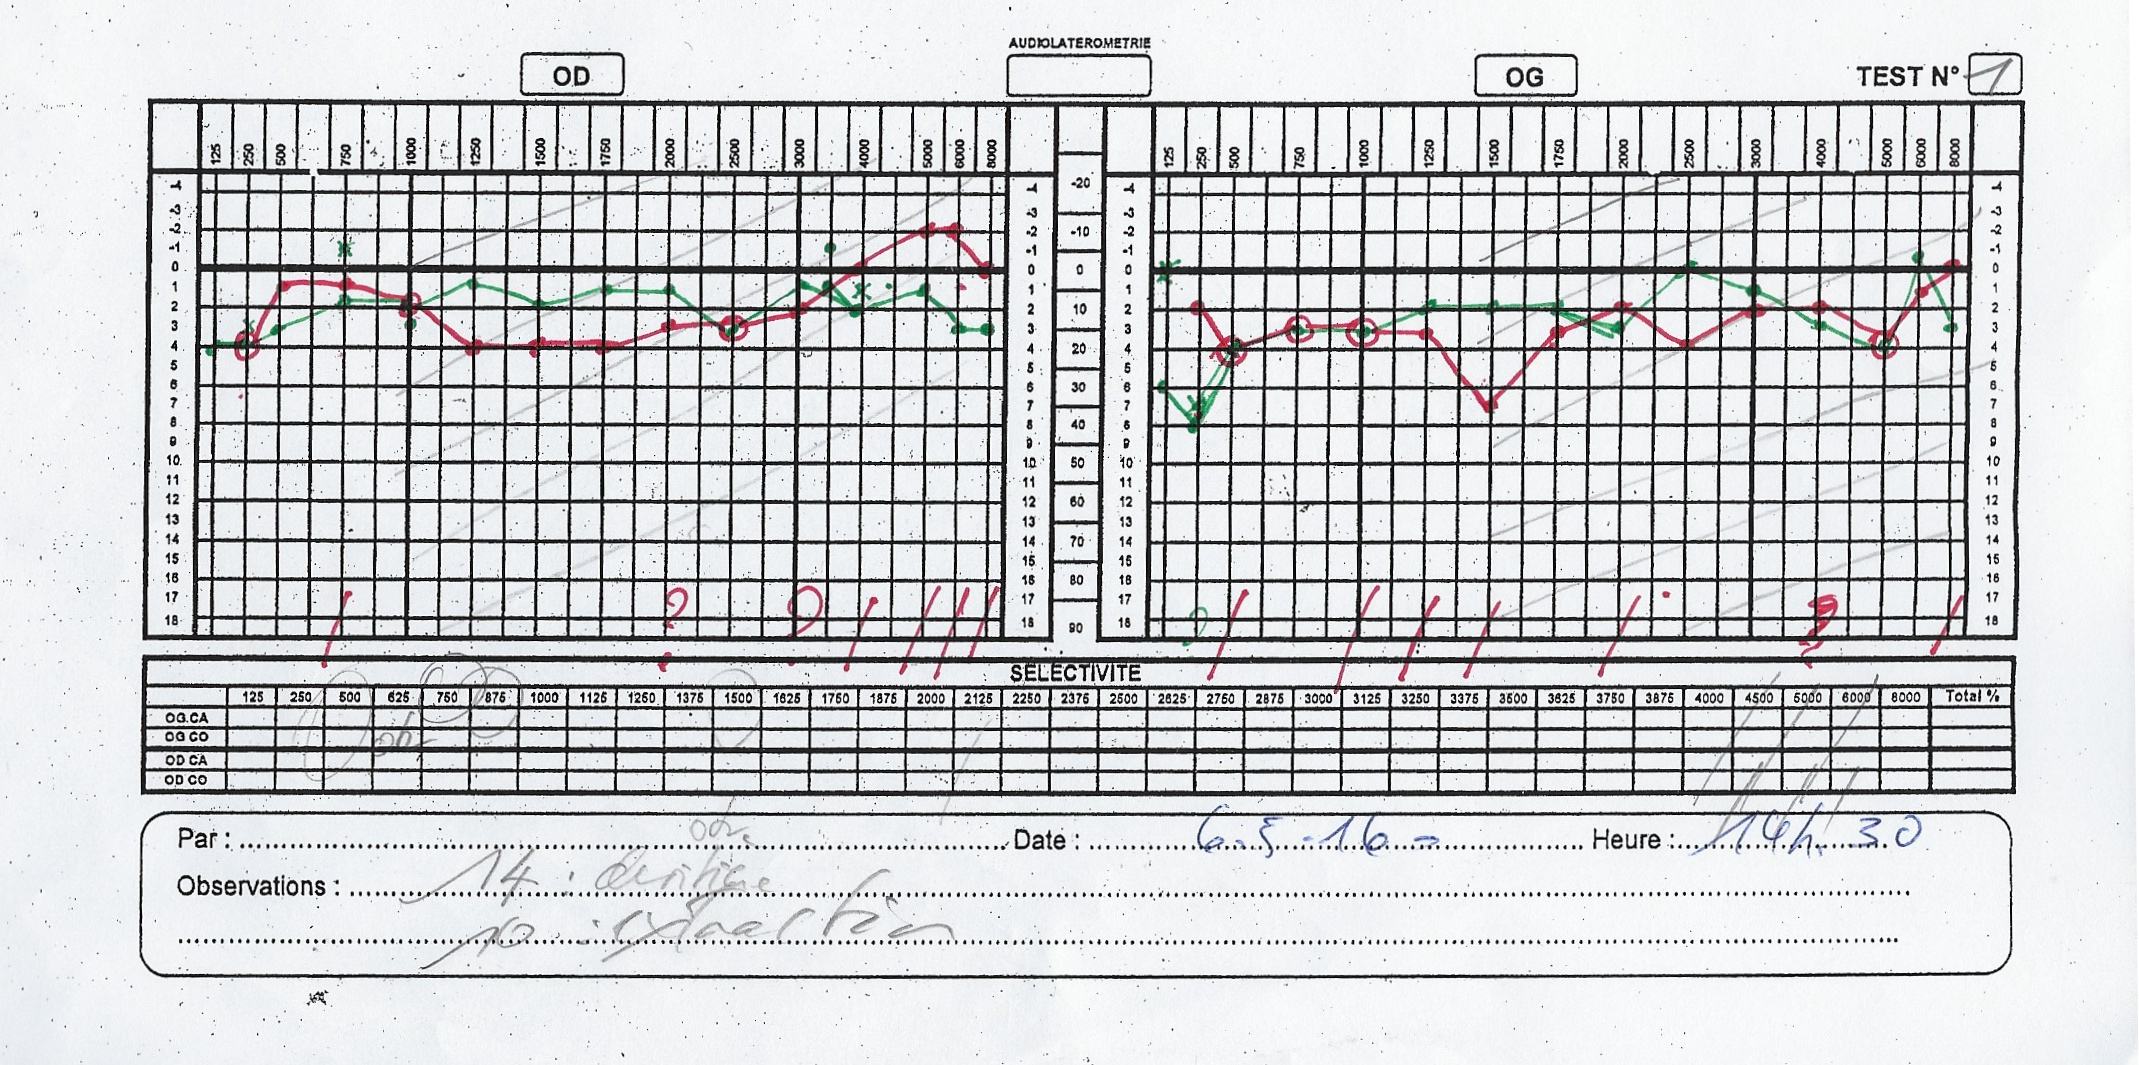
\includegraphics[scale=0.1,bb = 0 0 200 100, draft, type=eps]{PatientV1.jpg}}}
%}
%\end{figure}


\chapter{Etude avec utilisation du test Tomatis en clinique psychiatrique.}
Nous savons que la musicothérapie est de plus en plus intégrée dans
les milieux psychiatriques. Nous avons choisi ce terrain d'étude car 
nous  travaillons dans ce domaine  à temps partiel comme musicothérapeute.
\section{Cadre de travail}
 La Privatklinik
de Meiringen est  spécialisée en
addictologie dans le canton de Berne. Elle dispose d'une capacité de 195 lits, 33 médecins et
psychologues, secondés par 177 soignants qui assurent le suivi du
patient. Regula Lehman, musicothérapeute à temps complet, et nous-même avons
collaboré  pour l'organisation de la mise en place de l'étude. Celle-ci porte sur un même type de
population dans le contexte et cadre  précis d'une prise en charge globale
par les médecins, les psychologues, les physiothérapeutes,
ergothérapeutes et les divers ateliers de créativité proposés dans
cette clinique. Nous avons principalement travaillé avec des
pathologies comme celles du burnout, de la dépendance et de la
dépression, ceci dans une tranche d'âge de 20 à 60 ans, masculin et
féminin quasi égale. 
\section{Organisation d'étude}
Au préalable, nous avons fait circuler une
feuille d'information pour expliquer notre démarche d'évaluation sur
l'hypothèse de la transformation de l'écoute du patient lors de son
séjour en thérapie. \emph{Information für Mitwirkende an der klinischen
Studie\  "Evaluierung des aktiven Hörvermögens" }. 

\paragraph{Privatklinik von Meiringen}

Information für Mitwirkende an der klinischen Studie
« Evaluierung des aktiven Hörvermögens »


Sehr geehrte Damen und Herren,

Herzlichen Dank für Ihr Interesse an dieser Studie !

Wozu dient diese Studie und weshalb werden Sie um eine Teilnahme gebeten ?

Während Ihrem Klinikaufenthalt  in der Privatklinik von Meiringen werden Sie im Kontext 
unseres multidisziplinären Teams verschiedene Therapien besuchen, unter anderem auch die Musiktherapie. Bei der vorliegenden Studie möchten wir untersuchen, wie sich die Musiktherapie auf Ihr Zuhörvermögen auswirkt.
Musiktherapie ist eine gut erforschte Intervention im Bereich des Depressions und Burnouts, da Sie ein relativ neues Berufsfeld ist, gibt es noch viel Forschungspotential.
Das Hörtest konnte sich als ein Instrument erweisen, um die Veränderung des Gehörs des Patienten bei einer Musiktherapiebehandlung zu beweisen. Die Verbindung dieses Ansatzes mit der Musiktherapie ist noch nicht erforscht und daher soll dieser Ansatz wissenschaftlich näher untersucht werden.
Wenn Sie keine Musiktherapie besuchen aber Interesse für diese Studie haben, sind Sie herzlich eingeladen, dieses Test zu tun. Im Rahmen under MAS brauchen wir unbedingt eine Kontrollgruppe.

Wie sieht eine Teilnahme an der Studie aus ?

Die Untersuchung erfolgt sehr einfach in mehreren Schritten.
Zu Verfügung steht ein Apparat, mit dem sich spezifische Hörtests durchführen lassen.
Allgemein Verlauf des Tests :  
Sie hören einen sehr leisen Ton mit Zuhörern zu und werden ihn entweder mit der rechten  oder linken Hand  signalisieren. Das dauert ungefähr 30 Minuten.
Es wird zwei Tests geben : ein vor der Therapie und ein nach der Therapie.
Wir bitten Sie auch, eine kleine Fragebogen zu erfüllen.


Falls Sie Fragen haben, dürfen Sie sich gerne via E-Mail melden : valerie.gaillard\@gmx.ch

Wir bedanken uns herzlich für Ihre Zeit und die Teilnahme an dieser Studie.


Valérie Gaillard

 Le matériel utilisé : une table, deux chaises, l'appareil
test Hearing et les écouteurs aériens et osseux, un crayon, deux
feutres ( rouge et bleu), une feuille avec la grille de fréquences à
remplir.

ZhdK : Upgrade MAS Klinische Musiktherapie 15-17

 \section{Contact avec les patients}
 
 Regula Lehman a pu
préparer  les patients avec une explication préalable. Ensuite,
ceux-ci ont signé officiellement à chaque fois leur
accord pour cette participation  \emph{"Eine schriftliche Einbewilligung zum
Test"} avant de passer ces tests dont nous nous sommes occupées.
A Regula Lehmann  \footnote{Regula
  Lehmann, musicothérapeute  à 90\%  à la clinique de Meiringen} incombait la
prise en charge des séances en musicothérapie. Nous n'avons pas pu
toujours conserver cette configuration et nous avons dû suivre parfois
ponctuellement ou pendant le temps imparti certains patients en
musicothérapie. Par contre, le travail des tests était de notre ressort.  Nous avons organisé deux groupes, un témoin, sans
musicothérapie et un autre avec. Nous avions projeté d'en avoir
10 à chaque fois, mais ce ne fut pas simple de réunir ce
chiffre. Nous étions dépendants de leur entrée en clinique et de leur
sortie, après 4 semaines de thérapies, ce qui correspond à la durée
d'un séjour moyen dans cet établissement.


\begin{itemize}
	\item 10 patients testés, groupe A en musicothérapie : un
          premier test avant leur prise en charge en musicothérapie;
          puis un deuxième test \textdegree{} : après 4 semaines de
          clinique.
	\item 10 patients testés, groupe B de contrôle qui est un groupe sans musicothérapie,
	toujours dans le même contexte, c.à.dire la clinique, le suivi et les mêmes protocoles que l'autre groupe. Un premier test avant
	le début des autres thérapies puis un deuxième test, après 4 semaines. 
	Les tests ont été faits en avril, mai, juin, juillet, septembre et octobre 2017.
	Nous avons réalisé en tout 40 tests d'écoute Tomatis. 
	Précision importante : Pour cette étude, nous avons intentionnellement exclu la thérapie avec les musiques traitées et appliquées avec Tomatis, en nous restreignant  à ce lieu où l'application de cette forme de thérapie n'existe pas.
	Durée des tests : Chaque test Tomatis a une durée  moyenne de 50 à 60  minutes par patient. Pour chacun, nous avons donc réalisé en tout deux heures de tests d'écoute avec un entretien, et leur avons demandé en plus de remplir le questionnaire WHOQOL (20mn).
\end{itemize}

\section{Le WHOQO-Bref}

Nous avons utilisé et fait en parallèle le test WHOQO-Bref avant et
après pour avoir une variable supplémentaire pour confirmer en
parallèle supposée de l'action de la musicothérapie sur une éventuelle modification de l'écoute.  C'est une
version test de 1997 issue du Programme sur la santé mentale,
Organisation mondiale de la santé, Genève. Il y a 26 questions, que le
patient a rempli lui-même en présence du thérapeute, avant le test
d'écoute. La durée pour les remplir a varié de 8 à 10 minutes en
moyenne.  Il a eu 26 tests WHOQO-Bref.
Il y a quatre domaines testés : physique, psychologique, relations sociales et environnement.
\begin{enumerate}
	\item  Le domaine de la perception physique comprend l' activité quotidienne// la dépendance et/ou l'assistance médicale// la fatigabilité, l'énergie//la mobilité// la douleur// le sommeil// la capacité de travail//
	
		 \item Le domaine psychologique :  image de soi, apparence// ressentis positifs et négatifs// estime de soi// spiritualité, croyances personnelles, religion// mémoire et concentration, apprentissage, pensée.
		
			\item Le domaine des relations sociales : relations personnelles// soutien social// vie sexuelle.
			
			\item Le domaine de l'environnement : l'environnement domestique et  physique (pollution, bruit, trafic, climat)// la situation financière//  la liberté, la sécurité physique et morale// l'accessibilité et qualité de la santé// les opportunités de détente, loisirs et d'acquisition d'informations// le transport// 
		\end{enumerate}
		
	


 \section{Les tests d'écoute} 	
 
 \paragraph{Le test d'écoute Tomatis est une traduction graphique de l'écoute, elle permet d'objectiver la qualité de l'écoute.} 
 
  \begin{enumerate}
 	\item les seuils d'écoute
 	\item le son : dB, 
 	\item le volume de $-20$ à 90 % finesse typo: le signe moins des mathématiques.
 	\item les fréquence, de 125 à 8000.   \label{chapitre 6.2t} % mets une étiquette plus
 	% ``parlante'' stp, genre ``parametres_test_ecoute''.
 	\item la courbe, par l'observation des courbes d'écoute relevées
 	en comparaison avec la courbe dite idéale : équilibre,
 	déséquilibre, harmonie, disharmonie.  
 	\item équilibre, déséquilibre graphique entre les deux oreilles et entre les deux courbes mesurées par oreille: observation des croisements, des parallèles, des
 	écarts importants entre les courbes aériennes et osseuses\footnote{Remarque :
 		Un carré sur le graphique représente une différence de 5dB en
 		volume.}.
 	\item une modification perçue ou non comme évolutive lors des transformations graphiques de courbes
 	\item  Informations croisées avec les informations récoltées   par les 3 zones du test d'écoute: ........
 	\item une constatation de la posture d'écoute et de la qualité de
 	la voix. La voix se caractérise par son volume, son timbre, sa mélodie et son langage. 
 	
 	Nous suggérons de nous référer aux différents résultats des tests de et par la voix qui ont été faits pour tenter de déterminer un état dépressif ( Test et échelle d'Hamilton). Les chercheurs de l'université de Maryland en 2004, en émettant l'hypothèse de la modification de l'articulation vocale lors d'état dépressif ( on sait que la dépression provoque des changements  neuro-physiologiques) ont révélé lors du 168ème Congrès de la Société américaine d'acoustique, que les caractéristiques vocales se trouvaient modifiées lors de sentiments dépressifs\footnote{https://www.lci.fr/sante/et-si-on-diagnostiquait-la-depression-avec-un-test-vocal-sur-smartphone-1562728.html.}.
 		
 	
 	
 Nous pouvons faire ainsi le descriptif général de la voix d'un patient dépressif :
 	\begin{enumerate}
 		\item le volume : basse intensité
 		\item la mélodie : monotone, sans modulation
 		\item le timbre : mauvaise qualité due à une pertes des harmoniques
 		\item le langage : difficulté d'élocution
 	\end{enumerate}
 	
 		
 	
 	
 	
 	\section{Les graphiques}
 	
 	....
 	\section{Les résultats}
 	
 	....
 	
 	
 	
 \section{Les résultats et réflexions}	
Le manque de temps a été le principal facteur  réducteur
de tests valables, les départs imprévus des patients, et/ou leur
absence momentanée ( visite du psychologue, maladie, etc.). rajoutés au peu de temps de travail( 10\% )ainsi qu'à la
contingence difficile due à la distance séparant Genève du lieu de travail ( Meiringen)
: comment planifier un départ imprévu d'un patient !? il a fallu parfois
faire trois heures de route pour effectuer les tests finaux d'un ou deux
patients.
  
Par conséquent,  de nombreux tests sont restés 
incomplets et n'ont pu
être validés car ils ne remplissaient pas toutes les conditions requises.  En définitive, sur 40 tests d'écoute Tomatis et 26 tests
WHOQO-Bref, nous avons choisi de ressortir l'étude pour le groupe A de
5 patients effectifs en musicothérapie, tests complets, et le groupe
témoin B de 5 patients sur 9 effectifs, sans musicothérapie et tests
complets. 
 

  
\paragraph{Les résultats}
  
  De manière très générale, les résultats obtenus ne
  sont pas significatifs.  La prise en charge en musicothérapie a eu lieu
  une fois par semaine pendant une heure, ce qui semble trop court pour observer un changement important. Nous pourrions émettre la supposition suivante :  est-ce qu'un un travail journalier, régulier aurait été indiqué pour des résultats plus rapidement visibles avec le test?
  Est-ce qu'une immersion plus intensive en musicothérapie transformerait l'écoute des patients ? 
   En comparaison avec des
  modifications importantes de courbes des tests observées généralement  lors d' une écoute
  régulière de deux heures par jour de musique pendant 15 jours, --en référence à l'entrainement des muscles de l'oreille chez Tomatis, qui, nous le rappelons, est une pédagogie de l'écoute--, il aurait été intéressant de pouvoir faire cette étude comparative dans cette clinique. Ainsi, nous aurions pu éventuellement mettre en avant  l'absolue nécessité de créer et d'instaurer systématiquement la musicothérapie dans de nombreuses institutions mais aussi  de la développer beaucoup plus intensément  si elle est déjà existante.
  Nous sommes clairement en présence d'une ébauche d'études, avec des pistes
  suggérées. Ce travail ne peut être en aucun cas considéré comme
  quantitatif.  Nous avons ainsi pris l'option de nous tenir à une
  observation, celle de la transformation de l'écoute. Nous n'approfondirons pas l'évolution des diagnostics des différentes
  pathologies des patients.  (dépression, Burn out et dépendance.)
  
  A fortiori, relevons le cas fort intéressant  d'une patiente du groupe B( sans
  musicothérapie) : 
surprise d'apprendre par le premier test que la musique pouvait l'aider
  dans sa thérapie, celle-ci s'est mise à écouter assidûment du Mozart pendant la période de son séjour, entre le 1° test et le second test.  Les résultats
  graphiques obtenus lors de sa sortie sont clairement significatifs
  et sont en concordance avec le WHOQ-Bref. 
  ......



   
   
   
   
  \end{enumerate}







\paragraph{Hypothèse}

Est-ce possible d'évaluer un travail musicothérapeutique au moyen
d'un test d'écoute?

Est-ce que le processus d'écoute en musicothérapie améliore la capacité
d'écoute ?

Est-ce que les test auditifs avant et après la musicothérapie permettent
de visualiser l'action de la musicothérapie?

\paragraph{Y-a-t-il une modification de l'écoute du patient après une prise
en charge en musicothérapie ?}

\paragraph{Est-ce que les résultats ( = un changement dans l'écoute) d'une prise
en charge musicothérapeutique peuvent être lisibles et visibles dans
un test d'écoute Tomatis ?}

Est-ce que ces résultats sont significatifs? 

\paragraph{Est-ce que l'écoute du patient s'est modifié ? si on a pu observer
une modification, dans quel sens va -t-elle ?}

Est-ce ce test valable ? est-ce que le contexte est suffisant pour
ressortir des résultats ?






\chapter{Hypothèse : Réflexions et interrogations}

\section{Evaluation du travail fait en musicothérapie : }

Apprendre à écouter, c'est un travail et des résultats peuvent être
visibles. Nous utilisons un outil qui est le son. Nous accompagnons
le patient d'un point A pour aller au point B : que s'est -il passé
dans son écoute? Nous pouvons apporter des résultats visibles et tangibles
d'une forme d'apprentissage de l'écoute, d'une transformation de la
perception.On se base sur un graphique résultant d'un test de reconnaissance
de sons qui permet de visualiser une transformation psychologique
de l'écoute. 
\begin{itemize}
\item Il y a des résultats : nous pouvons constater soit un changement,
un statisme, un apprentissage,ou un refus d'apprendre et de se transformer.
Ce sont des données qui peuvent servir à mieux comprendre le patient
et à l'accompagner dans son cheminement.
\item Des questions sous-jacentes peuvent émerger comme celles-ci :
\end{itemize}
\begin{enumerate}
\item Quelle est la part d' objectivité ? de subjectivité?
\item S'il n'y a pas de changement visible dans le test , quelles conclusions
peut-on en tirer ? le changement va-t-il toujours de pair avec le
patient? synchronisé ou différencié dans le temps?
\item Est-ce normatif? par cette démarche, il y a le risque de catégoriser
et de paralyser le patient dans son parcours. Mais, cela peut aussi
l'aider dans son travail, son évolution. Ces deux possibilités sont
intrinsèques à tous les tests.
\end{enumerate}
\begin{itemize}
\item Nous sommes confrontés de plus en plus à donner des rapports aux caisse-maladies.
S'il y a une constatation de changement, de progression, le résultat
n'enfermera pas le patient dans une catégorie psychologique, qui,
transmise à celles-ci, pourrait lui être négative pour la poursuite
de son cheminement professionnel, via la vie active. 
\item Est-ce que ce test pourrait être un outil pour les thérapeutes et
les patients ? 
\item Avoir un support réel, visible car graphique pourrait-il être d'une
quelconque utilité pour le patient et pour le thérapeute ?
\item Est-il possible, à partir de deux tests d'écoute, de tirer des hypothèses
sur l'impact du son, de la musicothérapie, du soin par le son, sur
un patient ?
\item Le patient reste au centre de nos préoccupations.
\item Serait-ce un moyen, une façon de démontrer par ce moyen simple (autre
que l'Irmfct) que représente le test d'écoute l'utilité de la musicothérapie
? et ainsi de permettre une plus large acceptation et diffusion de
ce type de thérapie dans plus de milieux hospitaliers ou autres ?
\end{itemize}

\section{La musicothérapie et la méthode Tomatis : }

%\begin{thebibliography}{10}
\bibitem{key-1}''Biologie Humaine , Principes d'anatomie et de physiologie'',
Elaine N.Marieb, 8ème édition, Pearson Education.

\bibitem{key-2}d Auriol (1996), \emph{La clé des sons, }Ed.Erès

\bibitem{key-3}Jean-Claude Ameisen (2013), \emph{Sur les épaules
de Darwin, Les battements du temps. }Ed\emph{.}Les liens qui libèrent

\bibitem{key-7}Silvia Bencivelli (2009),\emph{ Pourquoi aime-t-on
la musique?Oreille, émotion,évolution. }Ed.Belin.pour la science.

\bibitem{key-4}Simone Dalla Bella, Movement to Health Laboratory,
Université de Montpellier,lors de la XIIème Rencontre Cerveau-Esprit:
``Les rythmes'', 22 mars 2012, Sion, SUVA.

\bibitem{key-4}Rolando Omar Benenzon (2007)\emph{. La musicothérapie,
La part oubliée de la personnalité. }De Boeck

\bibitem{key-5}Emanuel Bigand (2012) \emph{Conférence, Musicothérapie
et Identité sonore.}Dijon, 6 avril 2012,\emph{ La musique comme outil
de stimulation cognitive. }In Richelle, (2013)\emph{Le cerveau mélomane
. }Belin

\bibitem{key-6}Isabelle Haugmard (2010) \emph{ABC de la thérapie
par les sons. }Michel Granch

\bibitem{Viret}Jacques Viret (2007) \emph{B. A-BA de la musicothérapie,}.
Pardès

\bibitem{key-9}Denis le Bihan \emph{Le cerveau de cristal, ce que
nous révèle la neuro-imagerie} (2012) Odile Jacob, sciences.

\bibitem{key-10}Antonio Damasio (2010) \emph{L'autre moi-même, les
nouvelles cartes du cerveau, de la conscience et des émotions }. Odile
Jacob,sciences.

\bibitem{key-12}Joseph-Marie Verlinde (1998) \emph{L'expérience interdite
.}Saint-Paul

\bibitem{key-13}L'essentiel, Cerveau et psycho (2011) \emph{Le cerveau
mélomane. }Revue de psychologie

\bibitem{key-14-1}Alfred Tomatis (1987) \emph{L'oreille et la voix.
}R. Laffont

\bibitem{key-2-1}Alfred Tomatis\emph{ }(1983)\emph{Vers l'écoute
humaine, }2ème Ed.Tome 2, Collection Science de l'éducation

\bibitem{key-3-1}Alfred Tomatis (1977) \emph{L'oreille et la vie,}
Ed.Robert Laffont

\bibitem{key-4-1}Alfred Tomatis (1972) \emph{De la communication
intra-utérine au langage humain, la libération d'Oedipe,} 5ème Ed.,\emph{
}Collection Science de l'éducation

\bibitem{key-5-1}Alfred Tomatis ((1989) \emph{Neuf mois au paradis,
histoires de la vie prénatale,} Ed.Ergo Press

\bibitem{key-6-1}Alfred Tomatis (1988)\emph{Les troubles scolaires,}
Ed.ErgoPress

\bibitem{key-3}Dominique Sandre, Docteur en médecine, spécialiste
en pédiatrie, conférence du 6 avril 2012, Dijon, \emph{Environnement
sensoriel du bébé dans un contexte hospitalier.}

\bibitem{key-1}Daniel Barenboim (2008), pianiste et chef d'orchestre,
\emph{La musique éveille le temps}. Ed.Fayard

\bibitem{key-2}Jean-Yves Bosseur (2005), \emph{Du Son au Signe, Histoire
de la notation musicale. }Ed. Alternatives

\bibitem{key-1}Emission''Envoyé spécial'', conçue et animée par
Pierre Lane

\bibitem{key-1}Patrick Dumas de la Roque ``L'écoute, c'est la vie'',
éd. Jouvence, trois Fontaines 

\bibitem{key-7}Fern Nevjinsky,\emph{ Adolescence, musique, Rorschach,
}, publication de l'Université de Rouen n\textdegree 215, source internet
décembre 2016.

\bibitem{key-1}E.Gendlin,\emph{ Focusing,} (2010) Ed. Pocket Evolution 

\bibitem{key-2}Felicitas Sigrist, \emph{Burnout und Musiktherapie,
Grundlagen, Forschungsstand und Praxeologie, }Ed. Zeitpunkt Musik,
Reichert Verlag Wiesbaden 2016

\bibitem{key-3}Hans-Helmut Decker-Voigt, S\emph{chulen der Musiktherapie,
}Ernst Reinhardt Verlag München Basel
\end{thebibliography}

\bibliographystyle{plainnat-fr}
\selectlanguage{french}
\bibliography{valbib}
\end{document}
